%\documentclass[graybox,envcountchap,sectrefs,default]{svmono}
\documentclass[a4paper,11pt]{extbook}

\usepackage{amsmath}
\usepackage{amssymb}
\usepackage{graphicx}
\usepackage{float}

%\usepackage[T1]{fontenc}
%\usepackage[charter]{mathdesign}
%\usepackage[varg]{txfonts}

\usepackage{geometry}
\geometry{verbose,tmargin=1.5cm,bmargin=1.5cm,lmargin=1.5cm,rmargin=1.5cm}

%\usepackage{geometry}
%\geometry{verbose,tmargin=3cm,bmargin=3cm,lmargin=3cm,rmargin=3cm}

% DRAFT SETTINGS: easier to read in dark mode
%\usepackage{cmbright}
%\renewcommand{\familydefault}{\sfdefault}

\usepackage[libertine]{newtxmath}
\usepackage[no-math]{fontspec}
\setmainfont{Linux Libertine O}

%\usepackage{fontspec}
%\setmainfont{FreeSerif}
%\setmonofont{FreeMono}
%\setmonofont{DejaVu Sans Mono}
\setmonofont{JuliaMono-Regular}

\usepackage{framed}

\usepackage{braket}
\usepackage{mhchem}

\setcounter{secnumdepth}{3}
\setcounter{tocdepth}{3}
\setlength{\parskip}{\smallskipamount}
\setlength{\parindent}{0pt}
\usepackage{setspace}
\onehalfspacing

\usepackage{minted}
% using DejaVu Sans Mono, we need to scale the font to smaller size to match
% the main font.
\newminted{julia}{breaklines,fontsize=\footnotesize}
\newminted{bash}{breaklines,fontsize=\footnotesize}
\newminted{text}{breaklines,fontsize=\footnotesize}

\newcommand{\txtinline}[1]{\mintinline[fontsize=\footnotesize]{text}{#1}}
\newcommand{\jlinline}[1]{\mintinline[fontsize=\footnotesize]{julia}{#1}}

\newmintedfile[juliafile]{julia}{breaklines,fontsize=\footnotesize}

\usepackage{float}
\newfloat{mintedfloat}{h}{lop}
\floatname{mintedfloat}{Listing}

% Using background color for minted environment
\usepackage{xcolor}
\definecolor{mintedbg}{rgb}{0.9,0.9,0.9}
\usepackage{mdframed}
\BeforeBeginEnvironment{minted}{
    \begin{mdframed}[backgroundcolor=mintedbg,%
        topline=false,bottomline=false,%
        leftline=false,rightline=false]
}
\AfterEndEnvironment{minted}{\end{mdframed}}

\usepackage{hyperref}

\usepackage{multicol}

\usepackage{makeidx}
\makeindex

\begin{document}

\title{Implementing Density Functional Theory Calculations}
\author{Fadjar Fathurrahman \\
Hermawan Kresno Dipojono}
\maketitle

\frontmatter

%\begin{dedication}

Untuk Mariya Al Qibtiya Nasution, istriku tercinta {\color{red}$\heartsuit$}

\end{dedication}





\include{foreword}
\preface

Importance of density functional theory

Implementation of density functional theory in various program packages (free and commercial)

Several books about density functional theories

The problem: not yet giving necessary details

This book is our humble attempt to demystifying several aspects of practical density functional
theory to beginners in the field.

Objective of this book: show the reader how to implement a density functional theory
for simple system containing only model potential (such as harmonic potential)
and to non-local pseudopotentials which are usually used in typical DFT calculations
for molecular and crystalline systems.

Outline of the book:
1d, 2d, 3d, Schrodinger equation, Poisson equation, Kohn-Sham equation for local
(pseudo)potentials, Kohn-Sham equation for nonlocal pseudopotentials.

This is for \textit{acknowledgments}.
 
\vspace{\baselineskip}
\begin{flushright}\noindent
Bandung,\hfill {\it Fadjar Fathurrahman}\\
month year\hfill {\it Hermawan Kresno Dipojono}\\
\end{flushright}



%%%%%%%%%%%%%%%%%%%%%%%acknow.tex%%%%%%%%%%%%%%%%%%%%%%%%%%%%%%%%%%%%%%%%%
% sample acknowledgement chapter
%
% Use this file as a template for your own input.
%
%%%%%%%%%%%%%%%%%%%%%%%% Springer %%%%%%%%%%%%%%%%%%%%%%%%%%

\extrachap{Acknowledgements}

Use the template \emph{acknow.tex} together with the document class SVMono (monograph-type books) or SVMult (edited books) if you prefer to set your acknowledgement section as a separate chapter instead of including it as last part of your preface.



\tableofcontents

\mainmatter

\chapter{An introduction to density functional theory}

Many-body (electrons-nuclei) Hamiltonian (in atomic unit):
\begin{equation}
\hat{\mathcal{H}} = 
- \sum_{I=1}^{N_{a}} \frac{1}{2M_{I}} \nabla^{2}_{I}
- \sum_{i=1}^{N_{e}} \frac{1}{2m} \nabla^{2}_{i}
+ \sum_{I=1}^{N_{a}} \sum_{J \neq I}^{N_{a}} \frac{Z_{I} Z_{J}}{\left| \mathbf{R}_{I} - \mathbf{R}_{J} \right|}
+ \frac{1}{2} \sum_{i=1}^{N_{e}} \sum_{j \neq i}^{N_{e}} \frac{1}{\left| \mathbf{r}_{i} - \mathbf{r}_{j} \right|}
- \sum_{I=1}^{N_{a}} \sum_{i \neq i}^{N_{e}} \frac{Z_{I}}{\left| \mathbf{R}_{I} - \mathbf{r}_{i} \right|}
\end{equation}

$\mathbf{R} = \left\{ \mathbf{R}_{I}, I=1,2,\ldots,N_{a} \right\}$

$\mathbf{r} = \left\{ \mathbf{r}_{i}, i=1,2,\ldots,N_{e} \right\}$


Many-body Schroedinger equation
\begin{equation}
\hat{\mathcal{H}}\, \Psi_{n}(\mathbf{R},\mathbf{r}) = \mathcal{E}_{n}\, \Psi_{n}(\mathbf{R},\mathbf{r})
\end{equation}


\begin{equation}
\Psi(\mathbf{R},\mathbf{r},t) = \sum_{n} \Theta_{n}(\mathbf{R},t) \Phi_{n}(\mathbf{R},r)
\end{equation}


$\Theta_{n}(\mathbf{R},t)$ are wave functions describing dynamics of nuclear subsystem in each one of
adiabatic electronic eigenstates $\Phi_{n} (\mathbf{R},r)$.

\begin{equation}
\hat{h}_{e} \, \Phi_{n}(\mathbf{R},\mathbf{r}) = E_{n}\,\Phi_{n}(\mathbf{R},\mathbf{r})
\end{equation}

Electronic Hamiltonian:
\begin{equation}
\hat{h}_{e} = \hat{T} + \hat{U}_{ee} + \hat{V}_{ne} = \mathcal{H} - \hat{T}_{n} - \hat{V}_{nn}
\end{equation}




Kohn-Sham equation \cite{Kohn1965} \index{Kohn-Sham equation}:
\begin{equation}
\left[ -\frac{1}{2}\nabla^2 + V_{\mathrm{KS}}(\mathbf{r})\right]
\psi_{i}(\mathbf{r}) = \epsilon_{i} \, \psi_{i}(\mathbf{r})
\end{equation}
with Kohn-Sham potential:
\begin{equation}
V_{\mathrm{KS}}(\mathbf{r}) = V_{\mathrm{ion}}(\mathbf{r}) +
V_{\mathrm{Ha}}(\mathbf{r}) + V_{\mathrm{xc}}(\mathbf{r})
\end{equation}

\begin{equation}
V_{\mathrm{Ha}}(\mathbf{r}) = \int\, \frac{\rho(\mathbf{r}')}{\mathbf{r} - \mathbf{r}'}\,\mathrm{d}\mathbf{r}'
\end{equation}

\begin{equation}
V_{\mathrm{ion}}(\mathbf{r}) = \sum_{I=1} \frac{Z_{I}}{\mathbf{r} - \mathbf{R}_{I}}
\end{equation}



\begin{thebibliography}{99.}%
\bibitem{Kohn1965} Test Kohn Sham
\end{thebibliography}

\chapter{Schroedinger equation in 1d}

The equation we want to solve is (in Hartree atomic unit):
\begin{equation}
\left[ -\frac{1}{2}\frac{\mathrm{d}^2}{\mathrm{d}x^2} + V(x) \right] \psi(x) = E\, \psi(x)
\end{equation}
with the boundary conditions:
\begin{equation}
\lim_{x \rightarrow \pm \infty} = 0
\label{eq:BC_isolated}
\end{equation}
%
We will discretize the wave function, potentials, and various spatial quantities using
regular grid within the finite computational interval
$\left[x_{\mathrm{min}}, x_{\mathrm{max}}\right]$. This computational interval should be choosen
such that the boundary condition \ref{eq:BC_isolated} approximately satisfied.

We will choose the grid points $x_{i}$, $i = 1, 2, \ldots$ as:
\begin{equation}
x_{i} = x_{\mathrm{min}} + (i-1)h
\end{equation}
where $N$ is the number of grid points and $h$ is the spacing between the grid points
is:
\begin{equation}
h = \frac{ x_{\mathrm{max}} - x_{\mathrm{min}} }{N-1}
\end{equation}

The following code can be used to initialize the grid points:

\inputminted[breaklines,fontsize=\scriptsize]{julia}{codes/1d/init_FD1d_grid.jl}


\section{Approximating second derivative}

With the following notation: $\psi_{i} = \psi(x_{i})$, we can use 3-point
finite difference to approximate second derivative of $\psi(x)$:
\begin{equation}
\frac{\mathrm{d}^2}{\mathrm{d}x^2} \psi_{i} =
\frac{\psi_{i+1} - 2\psi_{i} + \psi_{i-1}}{h^2}
\end{equation}


Take $\{ \psi_{i} \}$ as (column) vector, we can represent the second derivative operation
as matrix multiplication:
\begin{equation}
\vec{\psi''} = \mathbb{D}^{(2)} \vec{\psi}
\end{equation}
%%
where $\mathbb{D}^{(2)}$ is the second derivative matrix operator
\begin{equation}
\mathbb{D}^{(2)} = \frac{1}{h^2}
\begin{bmatrix}
-2  &  1  &  0  &  0  & 0 & \cdots & 0 \\
 1  & -2  &  1  &  0  & 0 & \cdots & 0 \\
 0  &  1  & -2  &  1  & 0 & \cdots & 0 \\
 \vdots  &  \ddots  &  \ddots  & \ddots  & \ddots  & \ddots & \vdots \\
 0 & \cdots & 0 & 1 & -2 & 1 & 0 \\
 0  &  \cdots  & \cdots & 0  & 1  & -2  & 1 \\
 0  &  \cdots  & \cdots & \cdots & 0  &  1  & -2 \\
\end{bmatrix}
\end{equation}

An example implementation can be found in file \txtinline{build_D2_matrix_3pt.jl}.

\inputminted[breaklines,fontsize=\scriptsize]{julia}{codes/1d/build_D2_matrix_3pt.jl}

Test with Gaussian function:
\begin{equation}
\psi(x) = \mathrm{e}^{-\alpha x^2}
\end{equation}
%
which second derivative can be calculated as
%
\begin{equation}
\psi''(x) = \left( -2 \alpha + 4\alpha^2 x^2 \right) \mathrm{e}^{-\alpha x^2}
\end{equation}
%
They are implemented in the following code
\begin{juliacode}
function my_gaussian(x; α=1.0)
    return exp(-α*x^2)
end

function d2_my_gaussian(x; α=1.0)
    return (-2*α + 4*α^2 * x^2) * exp(-α*x^2)
end
\end{juliacode}

\begin{figure}[H]
{\center
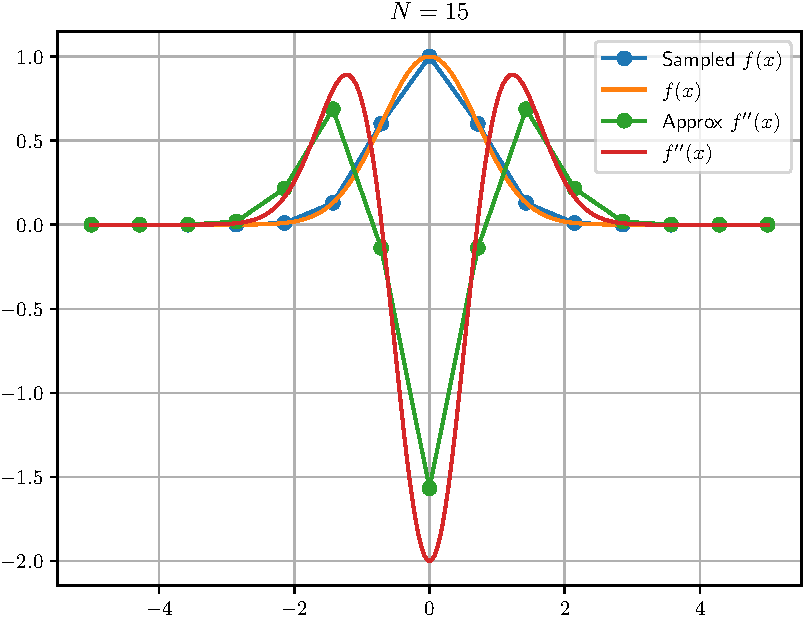
\includegraphics[scale=0.75]{codes/1d/IMG_gaussian_15.pdf}
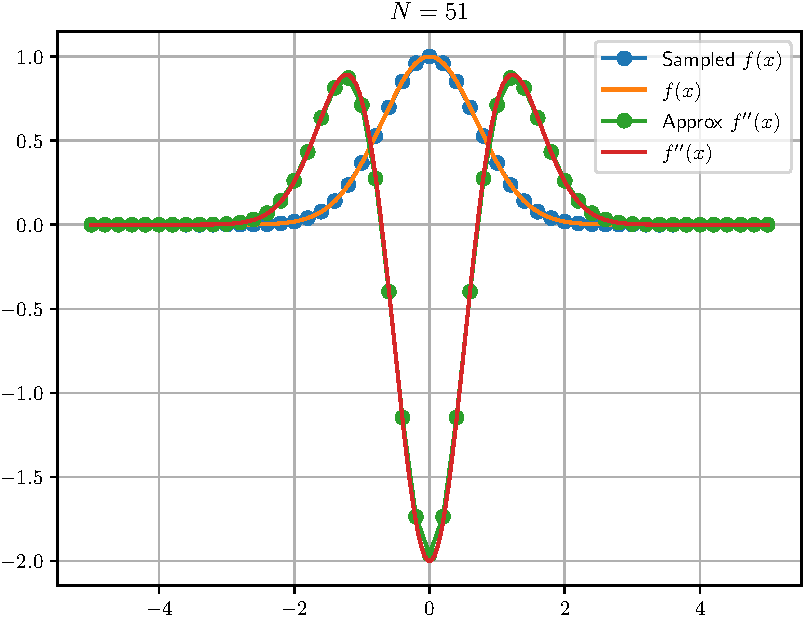
\includegraphics[scale=0.75]{codes/1d/IMG_gaussian_51.pdf}
\par}
\caption{Finite difference approximation to a Gaussian function and its second derivative}
\end{figure}


\section{Harmonic potential}

We will start with a simple potential with known exact solution, namely the harmonic potential:
\begin{equation}
V(x) = \frac{1}{2}\omega^2 x^2
\end{equation}

The Hamiltonian in finite difference representation:
\begin{equation}
\mathbb{H} = -\frac{1}{2}\mathbb{D}^{(2)} + \mathbb{V}
\end{equation}
where $\mathbb{V}$ is a diagonal matrix whose elements are:
\begin{equation}
\mathbb{V}_{ij} = V(x_{i})\delta_{ij}
\end{equation}


Code to solve harmonic oscillator:

\inputminted[breaklines,fontsize=\scriptsize]{julia}{codes/1d/main_harmonic_01.jl}

Compare with analytical solution.

Plot of eigenfunctions:

\begin{figure}[H]
{\center
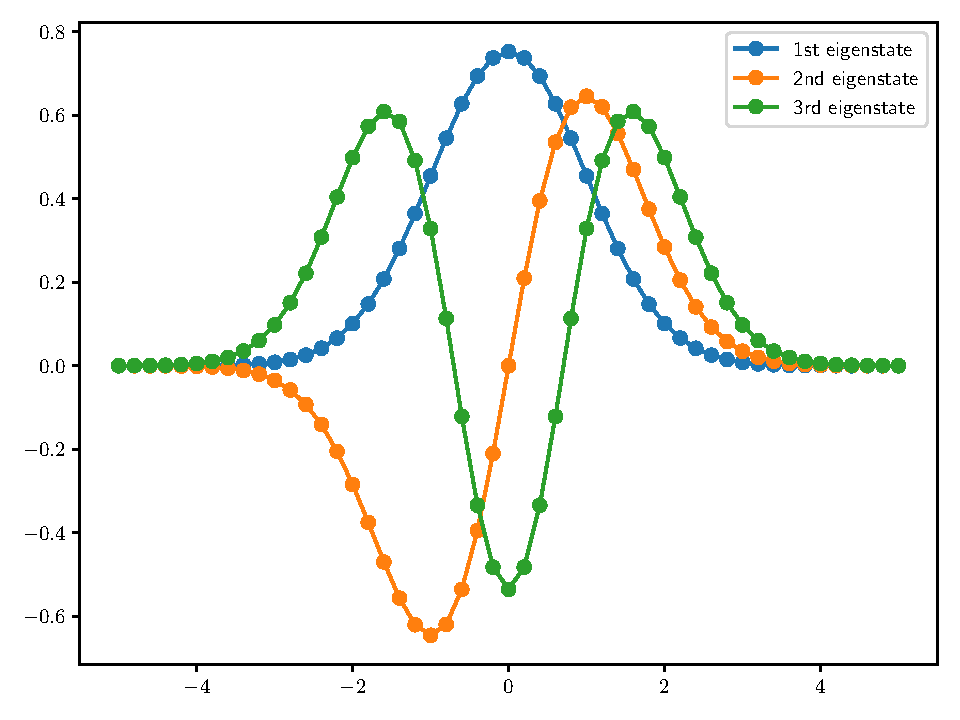
\includegraphics[scale=0.75]{codes/1d/IMG_main_harmonic_01_51.pdf}
\par}
\caption{Eigenstates of harmonic oscillator}
\end{figure}


\section{Higher order finite difference}

To obtain higher accuracy

Implementing higher order finite difference.


\section{Exercises}

Gaussian potential


\chapter{Schroedinger equation in 2d}

Now we will turn our attention to higher dimensions, i.e 2d.
The time-independent Schrodinger equation in 2d can be written as:
\begin{equation}
\left[ -\frac{1}{2}\nabla^2 + V(x,y) \right] \psi(x,y) = E\,\psi(x,y)
\label{eq:sch_2d}
\end{equation}
%
where $\nabla^2$ is the Laplacian operator:
%
\begin{equation}
\nabla^2 = \frac{\partial^2}{\partial x^2} + \frac{\partial^2}{\partial y^2}
\end{equation}



\section{Describing grid in 2d}

Now we have two directions $x$ and $y$. Our approach to solving the Schroedinger equation
is similar to the one we have used before in 1d, however several technical difficulties
will arise.

To describe the computational grid, we now need to specify
$x_{\mathrm{max}}, x_{\mathrm{min}}$ for the $x$-domain
and $y_{\mathrm{max}}, y_{\mathrm{min}}$ for $y$-domain. We also need to specify number of grid
points in for each x and y-directions, i.e. $N_{x}$ and $N_{y}$.
There are quite lot of variables.
For easier management, we will collect our grid related variables in one data structure or
\txtinline{struct} in Julia. A \txtinline{struct} in Julia looks very much like C-struct.
It also defines a new custom data type in Julia.

Our struct definition looks like this.
\begin{juliacode}
struct FD2dGrid
    Npoints::Int64
    Lx::Float64
    Ly::Float64
    Nx::Int64
    Ny::Int64
    hx::Float64
    hy::Float64
    dA::Float64
    x::Array{Float64,1}
    y::Array{Float64,1}
    r::Array{Float64,2}
    idx_ip2xy::Array{Int64,2}
    idx_xy2ip::Array{Int64,2}
    pbc::Tuple{Bool,Bool}
end
\end{juliacode}
%
An instance of \txtinline{FD2dGrid} can be initialized using the following constructor function:
%
\begin{juliacode}
function FD2dGrid( x_domain, Nx, y_domain, Ny )
    x, hx = init_FD1d_grid(x_domain, Nx)
    y, hy = init_FD1d_grid(y_domain, Ny)
    dA = hx*hy
    Npoints = Nx*Ny
    r = zeros(2,Npoints)
    ip = 0
    idx_ip2xy = zeros(Int64,2,Npoints)
    idx_xy2ip = zeros(Int64,Nx,Ny)
    for j in 1:Ny, i in 1:Nx
        ip = ip + 1
        r[1,ip] = x[i]
        r[2,ip] = y[j]
        idx_ip2xy[1,ip] = i
        idx_ip2xy[2,ip] = j
        idx_xy2ip[i,j] = ip
    end
    return FD2dGrid(Npoints, Nx, Ny, hx, hy,
      dA, x, y, r, idx_ip2xy, idx_xy2ip)
end
\end{juliacode}

A short explanation about the members of \txtinline{FD2dGrid} follows.
%
\begin{itemize}
%
\item \txtinline{Npoints} is the total number of grid points.
%
\item \txtinline{Nx} and \txtinline{Ny} is the total number of grid points
in $x$ and $y$-directions, respectively.
%
\item \txtinline{hx} and \txtinline{hy} is grid spacing in $x$ and $y$-directions,
respectively. \txtinline{dA} is the product of \txtinline{hx} and \txtinline{hy}.
%
\item \txtinline{x} and \txtinline{y} are the grid points in $x$ and $y$-directions.
The actual two dimensional grid points $r \equiv (x_{i},y_{i})$ are stored as
two dimensional array $r$.
%
\item Thw two integers arrays \txtinline{idx_ip2xy} and \txtinline{idx_xy2ip} defines
mapping between two dimensional grids and linear grids.
\end{itemize}


As an illustration let's build a grid for a rectangular domain
$x_\mathrm{min} = y_{\mathrm{min}}=-5$ and $x_\mathrm{max} = y_{\mathrm{max}}=5$
and $N_{x}=3$, $N_{y}=4$.
Using the above constructor for \txtinline{FD2dGrid}:
\begin{juliacode}
Nx = 3
Ny = 4
grid = FD2dGrid( (-5.0,5.0), Nx, (-5.0,5.0), Ny )
\end{juliacode}
%
Dividing the $x$ and $y$ accordingly we obtain $N_{x}=3$
grid points along $x$-direction
%
\begin{textcode}
julia> println(grid.x)
[-5.0, 0.0, 5.0]
\end{textcode}
%
and $N_{y}=4$ points along the $y$-direction
\begin{textcode}
julia> println(grid.y)
[-5.0, -1.6666666666666665, 1.666666666666667, 5.0]
\end{textcode}
%
The actual grid points are stored in \txtinline{grid.r}. Using the
following snippet, we can printout all of the grid points:
%
\begin{juliacode}
for ip = 1:grid.Npoints
    @printf("%3d %8.3f %8.3f\n", ip, grid.r[1,ip], grid.r[2,ip])
end
\end{juliacode}
%
The results are:
%
\begin{textcode}
  1   -5.000   -5.000
  2    0.000   -5.000
  3    5.000   -5.000
  4   -5.000   -1.667
  5    0.000   -1.667
  6    5.000   -1.667
  7   -5.000    1.667
  8    0.000    1.667
  9    5.000    1.667
 10   -5.000    5.000
 11    0.000    5.000
 12    5.000    5.000
\end{textcode}
%
We also can use the usual rearrange these points in the usual 2d grid rearrangement:
\begin{textcode}
[  -5.000,  -5.000] [  -5.000,  -1.667] [  -5.000,   1.667] [  -5.000,   5.000] 
[   0.000,  -5.000] [   0.000,  -1.667] [   0.000,   1.667] [   0.000,   5.000] 
[   5.000,  -5.000] [   5.000,  -1.667] [   5.000,   1.667] [   5.000,   5.000]
\end{textcode}
%
which can be produced from the following snippet:
%
\begin{juliacode}
for i = 1:Nx
    for j = 1:Ny
        ip = grid.idx_xy2ip[i,j]
        @printf("[%8.3f,%8.3f] ", grid.r[1,ip], grid.r[2,ip])
    end
    @printf("\n")
end
\end{juliacode}



\section{Laplacian operator}

Having built out 2d grid, we now turn our attention to the second derivative operator or
the Laplacian in the equation \ref{eq:sch_2d}.
There are several ways to build a matrix representation of the Laplacian, but we will
use the easiest one. 

Before constructing the Laplacian matrix, there is an important observation that
we should make about the second derivative matrix $\mathbb{D}^{(2)}$. We should note
that the second derivative matrix contains mostly zeros. This type of matrix that
most of its elements are zeros is called \textbf{sparse matrix}.
In a sparse matrix data structure, we only store its non-zero elements with specific
formats such as compressed sparse row/column format (CSR/CSC) and coordinate format.
We have not made use of the sparsity of the second derivative matrix
in the 1d case for simplicity. In the higher dimensions, however,
we must make use of this sparsity, otherwise we will waste computational resources 
by storing many zeros. The Laplacian matrix that we will build from
$\mathbb{D}^{(2)}$ is also very sparse.

Given second derivative matrix in $x$, $\mathbb{D}^{(2)}_{x}$,
$y$ direction, $\mathbb{D}^{(2)}_{x}$,
we can construct finite difference representation of the Laplacian operator
$\mathbb{L}$ by using
%
\begin{equation}
\mathbb{L} = \mathbb{D}^{(2)}_{x} \otimes \mathbb{I}_{y} +
\mathbb{I}_{x} \otimes \mathbb{D}^{(2)}_{y}
\end{equation}
%
where $\otimes$ is Kronecker product.
In Julia, we can use the function \jlinline{kron} to form the Kronecker product
between two matrices \jlinline{A} and \jlinline{B} as \jlinline{kron(A,B)}.

The following function illustrates the above approach to construct matrix
representation of the Laplacian operator.
\begin{juliacode}
function build_nabla2_matrix( grid::FD2dGrid )
    Nx = grid.Nx; hx = grid.hx
    Ny = grid.Ny; hy = grid.hy
    D2x = build_D2_matrix_9pt(Nx, hx)
    D2y = build_D2_matrix_9pt(Ny, hy)
    ∇2 = kron(D2x, speye(Ny)) + kron(speye(Nx), D2y)
    return ∇2
end
\end{juliacode}

The standard Julia library does not include definition for \jlinline{speye} function
but it can be implemented by the following definition.
\begin{juliacode}
speye(N::Int64) = sparse( Matrix(1.0I, N, N) )
\end{juliacode}

In the Figure \ref{fig:fd_gaussian_2d}, an example to the approximation of 2nd derivative
of 2d Gaussian function by using finite difference is shown.

\begin{figure}[h]
{\center
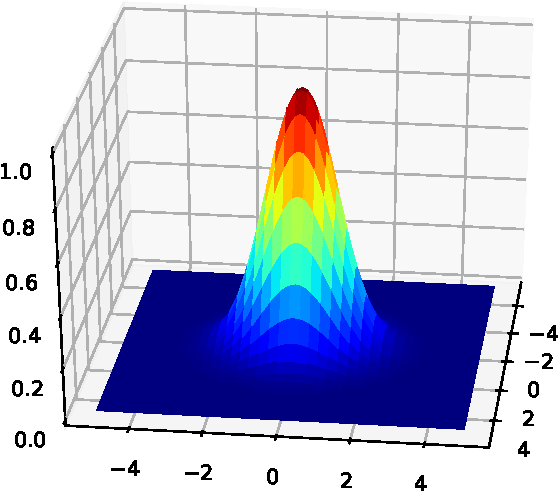
\includegraphics[width=0.6\textwidth]{../codes/FD2d/IMG_gaussian2d.pdf}
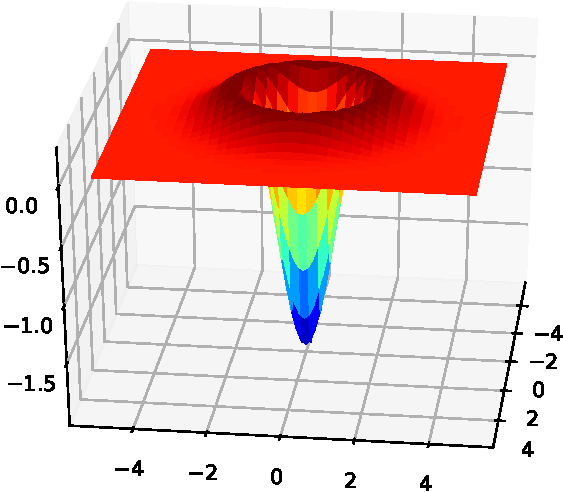
\includegraphics[width=0.6\textwidth]{../codes/FD2d/IMG_d2_gaussian2d.pdf}
\par}
\caption{Two-dimensional Gaussian function and its finite difference
approximation of second derivative}
\label{fig:fd_gaussian_2d}
\end{figure}


The following program is used to produce the figure.

\begin{juliacode}
using Printf
using LinearAlgebra
using SparseArrays
    
import PyPlot
const plt = PyPlot
    
include("FD2dGrid.jl")
include("build_nabla2_matrix.jl")
include("supporting_functions.jl")
    
function my_gaussian( grid; α=1.0 )
    Npoints = grid.Npoints
    f = zeros(Npoints)
    for i in 1:Npoints
        x = grid.r[1,i]
        y = grid.r[2,i]
        r2 = x^2 + y^2
        f[i] = exp(-α*r2)
    end
    return f
end
    
function main()  
    Nx = 75
    Ny = 75
    grid = FD2dGrid( (-5.0,5.0), Nx, (-5.0,5.0), Ny )
    
    ∇2 = build_nabla2_matrix( grid )
    
    fg = my_gaussian(grid, α=0.5)
    plt.clf()
    plt.surf(grid.x, grid.y, reshape(fg, grid.Nx, grid.Ny), cmap=:jet)
    plt.gca(projection="3d").view_init(30,7)
    fileplot = "IMG_gaussian2d.pdf"
    plt.savefig(fileplot)
    
    d2fg = ∇2*fg    
    plt.clf()
    plt.surf(grid.x, grid.y, reshape(d2fg, grid.Nx, grid.Ny), cmap=:jet)
    plt.gca(projection="3d").view_init(30,7)    
    fileplot = "IMG_d2_gaussian2d.pdf"
    plt.savefig(fileplot)
end
    
main()    
\end{juliacode}


\section{More about sparse matrices in Julia}

Using the function \jlinline{typeof} we can know the type of the variable
\jlinline{∇2} which was returned by the function \jlinline{build_nabla2_matrix}:
\begin{textcode}
julia> typeof(∇2)
SparseMatrixCSC{Float64,Int64}  
\end{textcode}
The \jlinline{CSC} part here is actually describe a certain format to store
a sparse matrix. It stands for \textbf{C}ompressed \textbf{S}parse \textbf{C}olumn
format. There are other formats as well: such as Compressed Sparse Row format (CSR),
coordinate list format (COO), and several others.

The CSC format stores a sparse matrix $\mathbf{A}$ with size $m \times n$
using three (one-dimensional) arrays (nzval, colptr, rowval).
Let Nnz denote the number of nonzero entries in $\mathbf{A}$.

The arrays nzval and rowval are of length Nnz, and contain the non-zero values
and the row indices of those values respectively.

An integer array colptr contains pointers to the beginning of each column in the
arrays nzval and rowval. Thus the content of colptr[i] is the position in
arrays nzval and rowval where the i-th row starts.
The length of colptr is n + 1 with colptr[n + 1] containing
the number colptr[1] + Nnz, i.e., the address in
nzval and rowval of the beginning of a
fictitious column m + 1.

The array colptr has one element per column in the matrix and encodes
the index in nzval where the given column starts. 
It may contain an extra end element which is set to Nnz.

Field names:
\begin{textcode}
julia> fieldnames(typeof(∇2))
(:m, :n, :colptr, :rowval, :nzval)  
\end{textcode}

From the documentation
\begin{juliacode}
struct SparseMatrixCSC{Tv,Ti<:Integer} <: AbstractSparseMatrix{Tv,Ti}
    #
    m::Int  # Number of rows
    #
    n::Int  # Number of columns
    #
    # Column j is in colptr[j]:(colptr[j+1]-1)
    colptr::Vector{Ti}
    #
    # Row indices of stored values
    rowval::Vector{Ti}
    # # Stored values, typically nonzeros
    nzval::Vector{Tv}
end
\end{juliacode}

Example 1:
\begin{equation}
A = \begin{bmatrix}
0  &  0  &  1.0 &  0.0 \\
5  &  8  &  0.0 &  0.0 \\
0  &  0  &  3.0 &  0.0 \\
0  &  6  &  0.0 &  0.0 \\
0  &  0  &  0.0 &  0.0
\end{bmatrix}
\end{equation}

\begin{textcode}
nzval = [5.0, 8.0, 6.0, 1.0, 3.0]
rowval = [2, 2, 4, 1, 3]
colptr = [1, 2, 4, 6, 6]
\end{textcode}

Example 2:
\begin{equation}
\mathbf{B} = \begin{bmatrix}
0  &  0  &  1  &  5 \\
5  &  0  &  0  &  0 \\
0  &  0  &  3  &  0 \\
0  &  0  &  0  &  0 \\
0  &  0  &  1  &  0 \\
5  &  0  &  0  &  6
\end{bmatrix}
\end{equation}

\begin{textcode}
nzval  = [5.0, 5.0, 1.0, 3.0, 1.0, 5.0, 6.0]
rowval = [2, 6, 1, 3, 5, 1, 6]
colptr = [1, 3, 3, 6, 8]
\end{textcode}

Example 3:
\begin{equation}
\mathbf{C} = \begin{bmatrix}
 -2  &  1  &  0  &  0  &  0 \\
  1  & -2  &  1  &  0  &  0 \\
  0  &  1  & -2  &  1  &  0 \\
  0  &  0  &  1  & -2  &  1 \\
  0  &  0  &  0  &  1  & -2
\end{bmatrix}
\end{equation}

\begin{textcode}
nzval  = [-2.0, 1.0, 1.0, -2.0, 1.0, 1.0, -2.0, 1.0, 1.0, -2.0, 1.0, 1.0, -2.0]
rowval = [1, 2, 1, 2, 3, 2, 3, 4, 3, 4, 5, 4, 5]
colptr = [1, 3, 6, 9, 12, 14]
\end{textcode}

Another way:
sparse(I,J,V) then constructs a sparse matrix such that S[I[k], J[k]] = V[k].

\section{Iterative methods for eigenvalue problem}

Now that we know how to build the Laplacian matrix, we now can build the Hamiltonian
matrix given some potential:
\begin{juliacode}
∇2 = build_nabla2_matrix( grid )
Ham = -0.5*∇2 + spdiagm( 0 => Vpot )
\end{juliacode}
Note that we have used sparse diagonal matrix for building the potential matrix by
using the function \txtinline{spdiagm}.
Our next task after building the Hamiltonian matrix is to find the eigenvalues
and eigenfunctions.
However, note that the Hamiltonian matrix size is large.
For example, if we use $N_x=50$ and $N_y=50$ we will end up with a Hamiltonian
matrix with the size of $2500$.
The use of \txtinline{eigen} method, as we have done in the 1d case,
to solve this eigenvalue problem is thus not practical.
Actually, given enough computer memory and time, we can use the function
\txtinline{eigen} anyway to find all eigenvalue and eigenfunction pairs of
the Hamiltonian, however it is not recommended
nor practical for larger problem size.

Typically, we do not need to solve for all eigenvalue and eigenfunction pairs.
We only need to solve for several eigenpairs with lowest eigenvalues. In a typical density
functional theory calculations, we only need to solve for $N_{\mathrm{electrons}}$ or
$N_{\mathrm{electrons}}/2$ lowest states, where $N_{\mathrm{electrons}}$ is the number
of electrons in the system.

In numerical methods, there are several methods to search for several eigenpairs
of a matrix. These methods falls into the category of \textit{partial or iterative
diagonalization methods}. Several known methods are Lanczos method, Davidson method,
preconditioned conjugate gradients, etc.
More detailed discussion about these methods are deferred to Appendix XXX.
We have prepared several implementation of iterative diagonalization methods
which can be used for black boxes for your convenience:
%
\begin{itemize}
\item \txtinline{diag_Emin_PCG}
\item \txtinline{diag_davidson}
\item \txtinline{diag_LOBPCG}
\end{itemize}
%
These functions have similar function signatures. They typically
need Hamiltonian, initial guess of wave function and preconditioner.
An example of \jlinline{diag_LOBPCG} is given below.
%
\begin{juliacode}
function diag_LOBPCG!(
  Ham, X::Array{Float64,2}, prec;
  tol=1e-5, NiterMax=100, verbose=false,
  verbose_last=false, Nstates_conv=0
)
\end{juliacode}
%
The three mandatory arguments are as follow:
%
\begin{itemize}
\item \jlinline{Ham}: the Hamiltonian matrix
\item \jlinline{X::Array{Float64,2}}: initial guess of eigenfunctions
\item \jlinline{prec}: the preconditioner
\end{itemize}

Almost all iterative methods need a good preconditioner to function properly.
We will use several ready-to-use preconditioners that have been implemented
in several packages in Julia such as incomplete LU and multigrid preconditioners.
In the next section we will describe a diagonalization method based
on nonlinear minimization as we apply it to a simple case of 2d harmonic
potential.


\section{Minimization approach: 2d harmonic potential}

We will test our implementation for solving Schroedinger equation for two
dimensional harmonic potentials:
%
\begin{equation}
V(x,y) = \frac{1}{2} \omega^2 (x^2 + y^2)
\end{equation}
%
This potential can be implemented in the following Julia code.
%
\begin{juliacode}
function pot_harmonic( grid::FD2dGrid; ω=1.0 )
    Npoints = grid.Npoints
    Vpot = zeros(Npoints)
    for i in 1:Npoints
        x = grid.r[1,i]
        y = grid.r[2,i]
        Vpot[i] = 0.5 * ω^2 *( x^2 + y^2 )
    end
    return Vpot
end
\end{juliacode}

This potential has the following analytic solutions for eigenvalues:
\begin{equation}
E_{n_{x} + n_{y}} = \hbar \omega \left( n_{x} + n_{y} + 1 \right)
\end{equation}
For each energy levels, we may have more than one possible combinations
of $n_x$ and $n_y$, for examples:

\begin{table}[h]
\centering
\begin{tabular}{|c|l|}
\hline
$E = n_x + n_y + 1$  &  Values of $n_x$ and $n_y$ \\
\hline
1                  &  (0,0) \\
2                  &  (1,0) (0,1) \\
3                  &  (2,0) (1,1) (1,1) \\
4                  &  (3,0) (0,3) (2,1) (1,2) \\
\hline
\end{tabular}
\end{table}

Our first task is to build the Hamiltonian. The step is very similar
to the one that we have done for 1d case:
\begin{juliacode}
Nx = 50
Ny = 50
grid = FD2dGrid( (-5.0,5.0), Nx, (-5.0,5.0), Ny )
∇2 = build_nabla2_matrix( grid )
Vpot = pot_harmonic( grid )
Ham = -0.5*∇2 + spdiagm( 0 => Vpot )
\end{juliacode}
Note that we have used \jlinline{spdiagm} instead of
\jlinline{diagm} when constructing the potential matrix.

\subsection{Orthonormalization}

We usually need to provide a guess solution or vectors to our eigensolver.
The guess vectors should be orthonarmalized properly before they can be supplied to
the eigensolver. There are several algorithms that can be used to orthonormalize
the vectors. One of them that will be used here is the Lowdin orthonormalization
which can be implemented in Julia as:
\begin{juliacode}
function ortho_sqrt( psi )
    Udagger = inv(sqrt(psi'*psi))
    return psi*Udagger
end
\end{juliacode}

As an example usage, here we start from random vectors and orthonormalize them
with \jlinline{ortho_sqrt}:
\begin{juliacode}
dVol = grid.dVol
Nstates = 3
Npoints = Nx*Ny
X = rand(Float64, Npoints, Nstates)
ortho_sqrt!(X, dVol)
\end{juliacode}

TODO: Gram-Schmidt ortho

TODO: check that the vectors are properly orthonormalized.


\subsection{Band energy functional and its gradient}

One method that can be used is diagonalize the Hamiltonian is based on the minimization
of band energy:
\begin{equation}
\min E\left[{\psi_{i}}\right] = \braket{\psi | H | \psi} - \sum_{ij}\lambda_{ij}\left(
\braket{ \psi_{i} | \psi_{j} } - \delta_{ij}
\right)
\end{equation}

The gradient of this expression is:
\begin{equation}
\frac{\partial H}{\partial \psi^{*}_{i}} = H\psi_{i} -
\sum_{j} \psi_{j} \braket{\psi_{j} | H | \psi_{i}}
\end{equation}
%
In Julia this can be implemented using the following function:
%
\begin{juliacode}
function calc_grad_evals!( Ham, ψ, g, Hsub )
    Nstates = size(ψ,2)
    Hψ = Ham*ψ
    Hsub[:] = ψ' * Hψ
    g[:,:] = Hψ - ψ*Hsub
    return
end
\end{juliacode}

\subsection{Steepest descent method}

The simplest method that we can apply to minimize the band energy functional is
the steepest descent method. This method can be described in the following steps:
\begin{enumerate}
\item Initialize random wave function: $\mathbf{X}$
\item Calculate $E$ for the given $\mathbf{X}$.
\item Calculate the gradient $\mathbf{g} = \nabla E$.
\item Set search direction $\mathbf{d} = -\mathbf{g}$.
\item Update wave function according to: $\mathbf{X} \leftarrow X + \alpha d$, where $\alpha$ is
a fixed step length. Orthonormalize $\mathbf{X}$.
\item Calculate $E$ for this updated $\mathbf{X}$ and compare it with the previous value.
\end{enumerate}

The following Julia code implements the steepest descent algorithm for minimizing band energy.
\begin{juliacode}
for iter = 1:NiterMax
    calc_grad_evals!( Ham, X, g, Hsub )
    d[:] = -g[:]
    # Update wavefunction
    X[:] = X + α_t*d
    ortho_sqrt!(X)
    Hr = Hermitian( X' * ( Ham*X ) )
    evals = eigvals(Hr)
    Ebands = sum(evals)
    devals = abs.( evals - evals_old )
    evals_old = copy(evals)
    nconv = length( findall( devals .< tol ) )
    diffE = abs(Ebands-Ebands_old)
    if nconv >= Nstates_conv
        IS_CONVERGED = true
        break
    end
    Ebands_old = Ebands
end
\end{juliacode}

Note we have calculate the current estimate the eigenvalues and band energy in the following
lines:
\begin{juliacode}
Hr = Hermitian( X' * ( Ham*X ) )
evals = eigvals(Hr)
Ebands = sum(evals)
\end{juliacode}

In the file \txtinline{main_harmonic_Emin_SD.kl} we
implement steepest descent algorithm
to find three lowest eigenstates of 2d harmonic potential.
Using the following parameters:
\begin{juliacode}
NiterMax = 5000
α = 3e-3
tol = 1e-6
\end{juliacode}
we obtain the results:
\begin{textcode}
evals[  1] =       0.9999999732 devals =   5.2402526762e-14
evals[  2] =       2.0000187702 devals =   1.1408453116e-07
evals[  3] =       2.0001656321 devals =   9.9907378681e-07  
\end{textcode}
which are close to the analytical solution. You might want to vary the number of eigenstates
that you want to search by setting higher values for the variable \jlinline{Nstates} to
higher than 3.

Despite its simplicity, the steepest descent method has several drawbacks.
The most prominent one is that it is very slow to converge. For this particular case
we have the following result.

\begin{textcode}
SD step     2258 =       5.0001854888   1.1198655e-06  nconv =     2
SD step     2259 =       5.0001843756   1.1131584e-06  nconv =     3
Emin_SD convergence: nconv =     3 in  2259 iterations
\end{textcode}

Note that the convergence is also dependent to the step
length parameter \jlinline{α}.

\subsection{Line minimization}

Line minimization:
\begin{juliacode}
Xc = ortho_sqrt( X + α_t*d )
calc_grad_evals!( Ham, Xc, gt, Hsub )
denum = real(sum(conj(g-gt).*d))
if denum != 0.0
    α = abs( α_t*real(sum(conj(g).*d))/denum )
else
    α = 0.0
end
\end{juliacode}

Implemented in the program \txtinline{main_harmonic_Emin_linmin.jl}.
Result using line minimization:
\begin{textcode}
linmin step      589 =       5.0000566204   1.4525395e-06  nconv =     2
linmin step      590 =       5.0000552040   1.4164238e-06  nconv =     3
Emin_linmin convergence: nconv =     3 in   590 iterations
  
Eigenvalues:
  
evals[  1] =       1.0000001750 devals =   3.4402208904e-07
evals[  2] =       2.0000051631 devals =   1.0311948540e-07
evals[  3] =       2.0000498659 devals =   9.6928218651e-07  
\end{textcode}


\subsection{Preconditioning}

Action of preconditioning:

\begin{juliacode}
Kg[:] = g[:] # copy
for i in 1:Nstates
    @views ldiv!(prec, Kg[:,i])
end
\end{juliacode}

ILU preconditioner based on kinetic operator:
\begin{juliacode}
prec = ilu(-0.5*∇2)
\end{juliacode}

Result using ILU preconditioner based on kinetic operator:
\begin{textcode}
linmin step       55 =       5.0000009960   1.2258080e-06  nconv =     2
linmin step       56 =       5.0000003689   6.2711750e-07  nconv =     3
Emin_linmin convergence: nconv =     3 in    56 iterations

Eigenvalues:

evals[  1] =       0.9999999739 devals =   6.0261565960e-07
evals[  2] =       1.9999999937 devals =   5.8729066055e-09
evals[  3] =       2.0000004014 devals =   1.8628935727e-08  
\end{textcode}

ILU preconditioner based on Hamiltonian operator:
\begin{juliacode}
prec = ilu(Ham)
\end{juliacode}

\begin{textcode}
linmin step       15 =       5.0000004295   3.2233493e-06  nconv =     2
linmin step       16 =       4.9999998058   6.2374058e-07  nconv =     3
Emin_linmin convergence: nconv =     3 in    16 iterations
  
Eigenvalues:
  
evals[  1] =       0.9999999787 devals =   1.2492943446e-07
evals[  2] =       1.9999998478 devals =   1.2682084205e-07
evals[  3] =       1.9999999792 devals =   3.7199030434e-07
\end{textcode}

Multigrid preconditioner
\begin{juliacode}
prec = aspreconditioner(ruge_stuben(Ham))
\end{juliacode}

\begin{textcode}
linmin step       15 =       5.0000010097   4.8543236e-06  nconv =     2
linmin step       16 =       4.9999999515   1.0581623e-06  nconv =     3
Emin_linmin convergence: nconv =     3 in    16 iterations

Eigenvalues:

evals[  1] =       0.9999999796 devals =   1.0151917307e-07
evals[  2] =       1.9999998532 devals =   1.9803365658e-07
evals[  3] =       2.0000001187 devals =   7.5860946458e-07
\end{textcode}


ILU0 preconditioner, in SPARSKIT.
\begin{juliacode}
prec = ILU0Preconditioner(Ham)
\end{juliacode}

\begin{textcode}
linmin step       64 =       5.0000041335   1.4349680e-06  nconv =     2
linmin step       65 =       5.0000030469   1.0865516e-06  nconv =     3
Emin_linmin convergence: nconv =     3 in    65 iterations

Eigenvalues:

evals[  1] =       1.0000001632 devals =   1.3899380646e-07
evals[  2] =       2.0000000485 devals =   6.1344835878e-08
evals[  3] =       2.0000028351 devals =   8.8621293415e-07
\end{textcode}


For testing purpose
\begin{juliacode}
prec = NoPreconditioner()
\end{juliacode}

Comparison of preconditioner size
\begin{textcode}
sizeof Ham  =       0.6372146606 MiB
sizeof prec =       6.9084167480 MiB  ILU kinetic
sizeof prec =       3.0494079590 MiB  ILU Hamiltonian
sizeof prec =       2.3046264648 MiB  AMG Ruge-Stuben
sizeof prec =       0.6372070313 MiB  ILU0
\end{textcode}


\subsection{Conjugate gradient}

Conjugate-gradient

\begin{textcode}
d = -Kg + β * d_prev
\end{textcode}

Polak-Ribiere formula
\begin{juliacode}
if iter != 1
    β = real(sum(conj(g-g_prev).*Kg))/real(sum(conj(g_prev).*Kg_prev))
end
if β < 0.0 β = 0.0 end
\end{juliacode}

CG using ILU$0$ (Ham)
\begin{textcode}
CG step       29 =       5.0000026056   2.8129344e-06  nconv =     2
CG step       30 =       5.0000011500   1.4555620e-06  nconv =     3
Emin_CG convergence: nconv =     3 in    30 iterations
  
Eigenvalues:
  
evals[  1] =       1.0000001156 devals =   1.4606434040e-07
evals[  2] =       2.0000002046 devals =   6.6796002196e-07
evals[  3] =       2.0000008298 devals =   6.4153765811e-07  
\end{textcode}


\subsection{Eigenfunctions}

\begin{juliacode}
ortho_sqrt!(X)
Hr = Hermitian( X' * (Ham*X) )
evals, evecs = eigen(Hr)
X[:,:] = X*evecs
\end{juliacode}

The eigenfunctions are shown in Figure \ref{fig:harm_2d_eigenfunctions}.

\begin{figure}[h]
{\centering
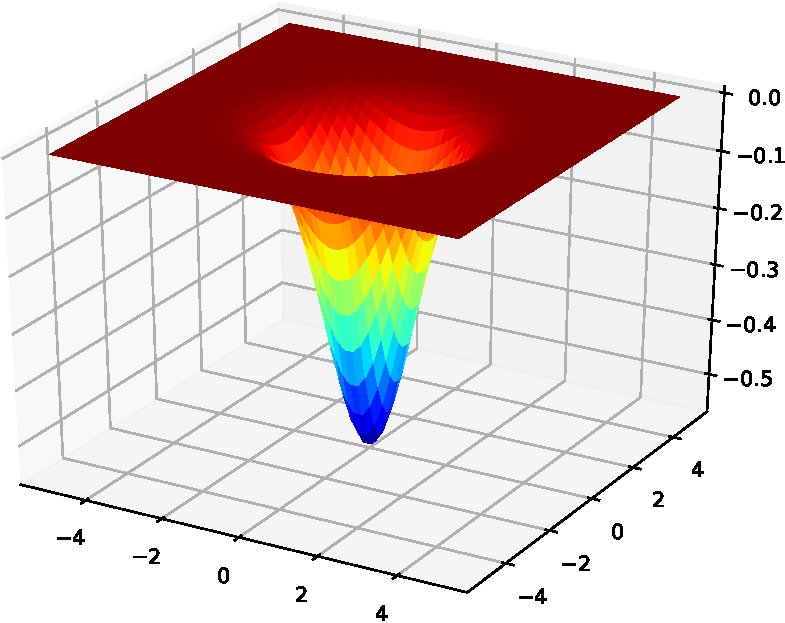
\includegraphics[width=0.4\textwidth]{../codes/sch_2d/IMG_harmonic_psi_1.pdf}\\
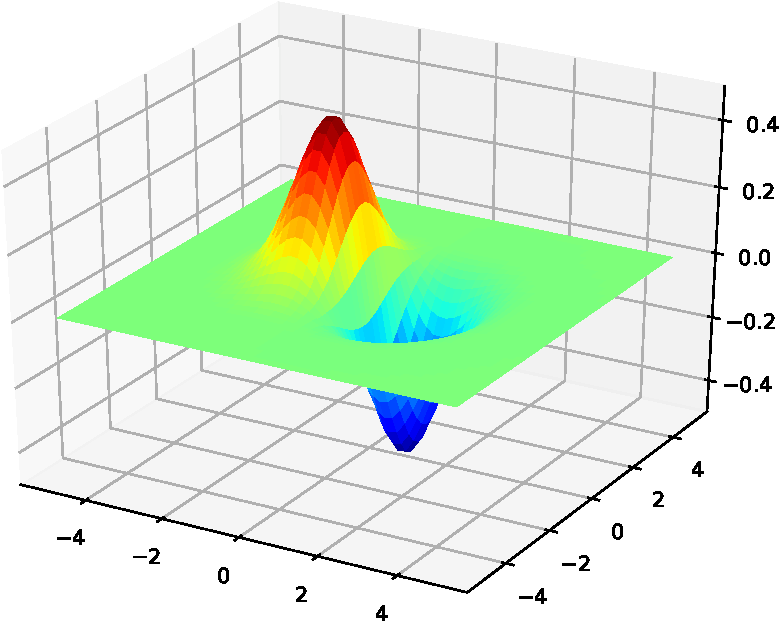
\includegraphics[width=0.4\textwidth]{../codes/sch_2d/IMG_harmonic_psi_2.pdf}%
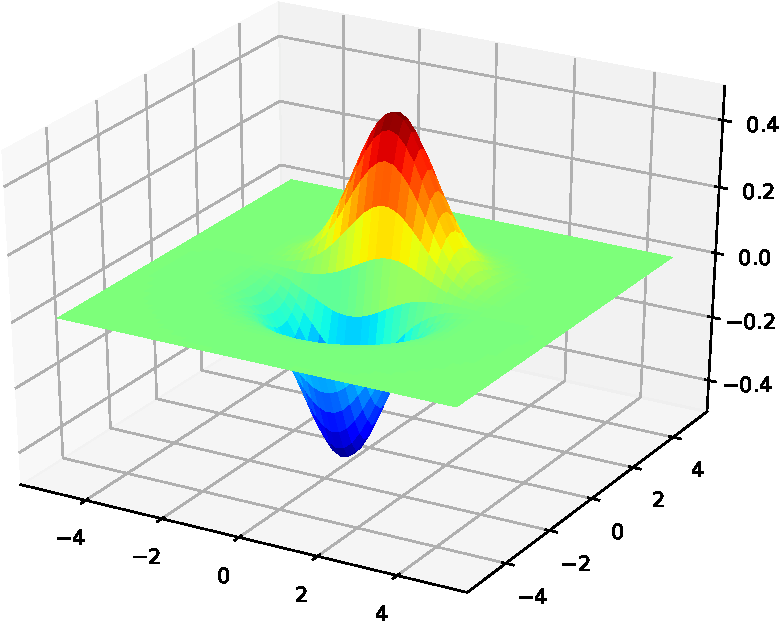
\includegraphics[width=0.4\textwidth]{../codes/sch_2d/IMG_harmonic_psi_3.pdf}
\par}
\caption{Visualization of eigenstates of 2d harmonic potential}
\label{fig:harm_2d_eigenfunctions}
\end{figure}

\section{Exercises}

2d Gaussian potential
\chapter{Schroedinger equation in 3d}

After we have considered two-dimensional Schroedinger equations, we are now ready for
the extension to three-dimensional systems. In 3d, Schroedinger equation can be
written as:
\begin{equation}
\left[ -\frac{1}{2}\nabla^2 + V(\mathbf{r}) \right] \psi(\mathbf{r}) = E\,\psi(\mathbf{r})
\end{equation}
where $\mathbf{r}$ is the abbreviation to $(x,y,z)$ and
%
$\nabla^2$ is the Laplacian operator in 3d:
\begin{equation}
\nabla^2 = \frac{\partial^2}{\partial x^2} + \frac{\partial^2}{\partial y^2} +
\frac{\partial^2}{\partial z^2}
\end{equation}

\subsection{Three-dimensional grid}

As in the preceeding chapter, our first task is to create a representation of 3d grid
points and various quantities defined on it. This task is realized using straightforward
extension of \txtinline{FD2dGrid} to \txtinline{FD3dGrid}.


Visualization of 3d functions as isosurface map or slice of 3d array.

Introducing 3d xsf


\subsection{Laplacian operator}

The Laplacian in 3d can be written as:
\begin{equation}
\mathbb{L} = \mathbb{D}^{(2)}_{x} \otimes \mathbb{I}_{y} \otimes \mathbb{I}_{z} +
\mathbb{I}_{x} \otimes \mathbb{D}^{(2)}_{y} \otimes \mathbb{I}_{z} +
\mathbb{I}_{x} \otimes \mathbb{I}_{y} \otimes \mathbb{D}^{(2)}_{z}
\end{equation}

The Julia code is also similar to the one we have used for the case of 2d:
%
\begin{juliacode}
const ⊗ = kron
function build_nabla2_matrix( grid )
  # ... SNIPPED
  # build D2x, D2y, and D2z matrices
  IIx = speye(grid.Nx)
  IIy = speye(grid.Ny)
  IIz = speye(grid.Nz)    
  ∇2 = D2x⊗IIy⊗IIz + IIx⊗D2y⊗IIz + IIx⊗IIy⊗D2z
  return ∇2
end
\end{juliacode}
%
The main difference is that we have used the symbol \txtinline{⊗} in place
of \txtinline{kron} function to make our code simpler. In Julia this symbol
can be entered by typing \txtinline{\otimes} in Julia console or text editors
that have been set up to use Julia extension and Unicode input.


\section{3d harmonic oscillator}

We hope that at this point you will have no difficulties to create your own
Schroedinger equation solver for 3d harmonic potential:
\begin{equation}
V(x,y,z) = \frac{1}{2}\omega^2 \left( x^2 + y^2 + z^2 \right)
\end{equation}

The analytic solution for the energy levels of this potential can be written as:
\begin{equation}
E_{n_{x} + n_{y} + n_{z}} = \hbar \omega \left( n_{x} + n_{y} + n_{z} + \frac{3}{2} \right)
\end{equation}
where $n_x, n_y, n_z$ are integers positive integers including zero.
%
For each energy level we have the following degeneracies:
\begin{equation}
g_{n} = \frac{(n + 1)(n + 2)}{2}
\end{equation}
where $n = n_x + n_y + n_z$.
%
For examples:
\begin{textcode}
n = n_x + n_y + n_z

n = 0: (1)(2)/2 = 1
n = 1: (2)(3)/2 = 3
n = 2: (3)(4)/2 = 6
\end{textcode}

The following is the result of \jlinline{diag_Emin_PCG}, for the 4 lowest eigenstates:
\begin{textcode}
CG step       12 =       8.9999996162 4.4341014e-06
evals[  1] =       1.4999999732, devals =   4.1020002284e-07
evals[  2] =       2.4999998628, devals =   1.0054977597e-06
evals[  3] =       2.4999998760, devals =   1.3278320172e-06
evals[  4] =       2.4999999042, devals =   1.6905715712e-06
iter 12 nconv = 4
Convergence is achieved based on nconv    
\end{textcode}
%
The obtained eigenvalues are close the the analytic solution.
Note that the we have 3 degenerate eigenstates.
You can try to vary the number of requested eigenstates to very that the degeneracies are
correct.


\section{Hydrogen atom}

\subsection{Coulomb potential and its singularity}

Until now, we only have considered simple potentials such as harmonic potential. Now we will
move on and consider more realistic potentials which is used in practical electronic calculations.

For most applications in materials physics and chemistry the external potential that is
felt by electrons is the Coulombic potential due to atomic nucleus. This potential has
the following form:
\begin{equation}
V(r) = -\sum_{I}^{N_{\mathrm{atom}}} \frac{Z_{I}}{\left|\mathbf{r} - \mathbf{R}_{I}\right|}
\end{equation}
where $R_{I}$ are the positions and $Z_{I}$ are the charges
of the atomic nucleus present in the system.
%
We will consider the most simplest system, namely the hydrogen atom $Z_{I}=1$, for which we have
\begin{equation}
V(r) = -\frac{1}{\left|\mathbf{r} - \mathbf{R}_{0}\right|}
\end{equation}
%
The following Julia code implement the H atom potential:
\begin{juliacode}
function pot_H_atom( grid; r0=(0.0, 0.0, 0.0) )
  Npoints = grid.Npoints
  Vpot = zeros(Npoints)
  for i in 1:Npoints
    dx = grid.r[1,i] - r0[1]
    dy = grid.r[2,i] - r0[2]
    dz = grid.r[3,i] - r0[3]
    Vpot[i] = -1.0/sqrt(dx^2 + dy^2 + dz^2)
  end
  return Vpot
end
\end{juliacode}

With only minor modification to our program for harmonic potential, we can solve the Schroedinger
equation for the hydrogen atom:
\begin{juliacode}
grid = FD3dGrid( (-5.0,5.0), Nx, (-5.0,5.0), Ny, (-5.0,5.0), Nz )
∇2 = build_nabla2_matrix( grid )
Vpot = pot_H_atom( grid )
Ham = -0.5*∇2 + spdiagm( 0 => Vpot )
prec = aspreconditioner(ruge_stuben(Ham))
Nstates = 1  # only choose the lowest lying state
Npoints = Nx*Ny*Nz
X = ortho_sqrt( rand(Float64, Npoints, Nstates) ) # random initial guess of wave function
evals = diag_LOBPCG!( Ham, X, prec, verbose=true )
\end{juliacode}

For the grid size of $N_{x}=N_{y}=N_{z}=50$ and using 9-point finite-difference approximation
to the second derivative operator in 1d we obtain the eigenvalue of -0.4900670759 Ha which
is not too bad if compared with the exact value of -0.5 Ha. We can try to increase the grid
size until we can get satisfactory result.

Note that there is a caveat when we are trying to use the Coulombic potential. This potential
is divergent at $r=0$, so care must be taken such that this divergence is not encountered in
the numerical calculation. In the previous code, we have tried to achieve this by using
choosing the numbers
$N_{x}$, $N_{y}$, and $N_{z}$ to be even numbers. This way, we avoid the evaluation of
the potential at the singular point of the Coulomb potential
(the point $\mathbf{r} = (0,0,0)$ in this
particular case).

\subsection{Pseudopotential}

In the many electronic structure calculations, it is sometime convenient to replace the
Coulomb potential with another potential which is smoother which we
will refer to as a \textbf{pseudopotential}. Not all smooth
potentials can do the job. The smooth potential should satisfy several requirements.
One of the most important requirement is that the smooth potential should have similar
scattering properties as the original Coulomb potential that it replaces.
This means that the potential should have posses similar eigenvalues as the
original Coulomb potential. Usually we don't try to reproduce all eigenvalue spectrum but only
the eigenvalues which belongs to the valence electrons. The valence electrons are
responsible for most chemically and physically important properties so this is an
acceptable approximation for most cases.

The theory and algorithms for constructing pseudopotentials are beyond the scope of
this book.
Most pseudopotentials are non-local by construction and this can make our program rather
complicated.
In this chapter we will focus on the so-called local pseudopotential. Practically, local
pseudopotentials pose no additional difficulties as the potentials that we have
considered so far. As an example of a pseudopotential, we will consider the following
local pseudopotential for hydrogen atom:
\begin{equation}
V_{\mathrm{H,ps}}(r) = -\frac{Z_{\mathrm{val}}}{r}
\mathrm{erf}\left( \frac{\bar{r}}{\sqrt{2}} \right) +
\exp\left( -\frac{1}{2}\bar{r}^2 \right)
\left( C_{1} + C_{2}\bar{r}^2 \right)
\label{eq:H_psp_GTH}
\end{equation}
where $\bar{r}=r/r_{\mathrm{loc}}$ and with the parameters $r_{loc}=0.2$, 
$Z_{\mathrm{val}}=1$, $C_{1}=-4.0663326$, and $C_{2}=0.6678322$.

The following Julia code implements this pseudopotential.
\begin{juliacode}
function pot_Hps_HGH( grid; r0=(0.0, 0.0, 0.0) )
  Npoints = grid.Npoints
  Vpot = zeros( Float64, Npoints )
  Zval = 1
  rloc = 0.2
  C1 = -4.0663326
  C2 = 0.6678322
  for ip = 1:Npoints
    dx2 = ( grid.r[1,ip] - r0[1] )^2
    dy2 = ( grid.r[2,ip] - r0[2] )^2
    dz2 = ( grid.r[3,ip] - r0[3] )^2
    r = sqrt(dx2 + dy2 + dz2)
    if r < eps()
      Vpot[ip] = -2*Zval/(sqrt(2*pi)*rloc) + C1
    else
      rrloc = r/rloc
      Vpot[ip] = -Zval/r * erf( r/(sqrt(2.0)*rloc) ) + (C1 + C2*rrloc^2)*exp(-0.5*(rrloc)^2)
    end
  end
  return Vpot
end
\end{juliacode}
Note that, you need to import \jlinline{erf} from the package \jlinline{SpecialFunctions}:
\begin{juliacode}
import SpecialFunctions: erf
\end{juliacode}
We also have been careful to not evaluate the term $Z_{val}/r$ by adding a check for the value of $r$.
If it is very small (close to zero, or smaller than $eps()$) then we are using the limiting
value of \ref{eq:H_psp_GTH} when $r \rightarrow 0$:
\begin{equation}
V_{\mathrm{H,ps}}(r) = -\frac{Z_{\mathrm{val}}}{r}
  \mathrm{erf}\left( \frac{r}{\sqrt{2}r_{\mathrm{loc}}} \right) + C_{1}
\end{equation}

\begin{equation}
V_{\mathrm{H,ps}}(\sqrt{2}r_{\mathrm{loc}} ) = -\frac{Z_{\mathrm{val}}}{r \sqrt{2}r_{\mathrm{loc}}}
  \frac{\mathrm{erf}(r)}{r} + C_{1}
\end{equation}

\begin{equation}
V_{\mathrm{H,ps}}(0) = -\frac{Z_{\mathrm{val}}}{\sqrt{2}r_{\mathrm{loc}}}
  \frac{2}{\sqrt{\pi}} + C_{1}
\end{equation}

The comparison of this potential and Coulomb potential can be seen in
Figure \ref{fig:compare_H_pspot}.
\begin{figure}[H]
{\centering
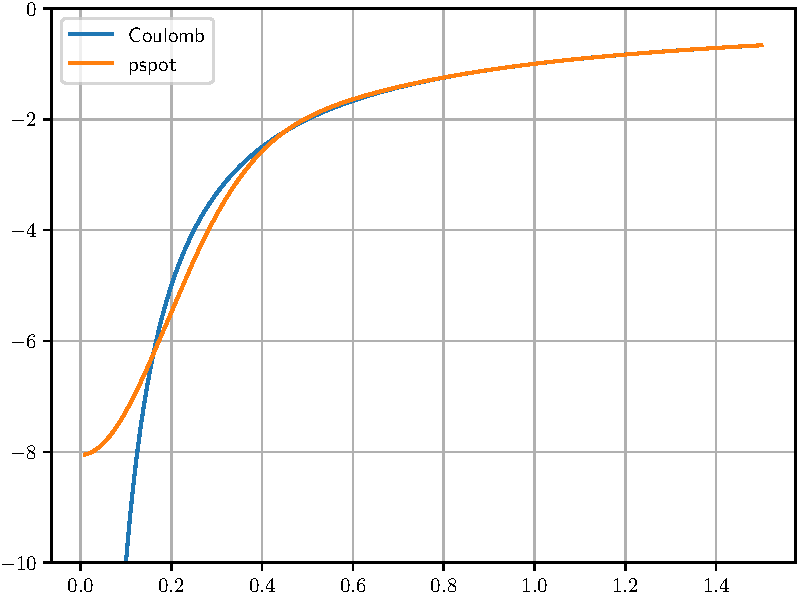
\includegraphics[width=0.65\textwidth]{../codes/sch_3d/IMG_H_Coulomb_vs_pspot.pdf}
\par}
\caption{Comparison Coulomb potential vs pseudopotential}
\label{fig:compare_H_pspot}
\end{figure}

The pseudopotential in \ref{eq:H_psp_GTH} is actually a special case of the more general
form of the local part of pseudopotential developed by Goedecker-Teter-Hutter (GTH):
\begin{equation}
V^{\mathrm{ps}}_{\mathrm{loc}}(r) = -\frac{Z_{\mathrm{val}}}{r}
\mathrm{erf}\left( \frac{\bar{r}}{\sqrt{2}} \right) +
\exp\left( -\frac{1}{2}\bar{r}^2 \right)
\left( C_{1} + C_{2}\bar{r}^2 + C_{3}\bar{r}^4 + C_{4}\bar{x}^6\right)
\label{eq:V_loc_GTH}
\end{equation}
GTH pseudopotentials also come with the nonlocal potential which is considerably more complicated
that the local one.
We will consider the case of nonlocal pseudopotentials in Chapter 7.
GTH pseudopotentials have are parameterized from density functional calculations for many elements
in the periodic table. 



\section{Exercises}

Compare the convergence of eigenvalue of hydrogen potential when using Coulomb potential
vs pseudopotential.

Higher eigenstates of H atom + visualization using Xcrysden

H2 molecule

He atom

LiH molecule
\chapter{Poisson equation}
\label{chap:poisson_3d}

\section{Conjugate gradient method}

In this section we will discuss a second type of equation
that is important in solving Kohn-Sham equation,
namely the Poisson equation. In the
context of solving Kohn-Sham equation, Poisson equation is used to
calculate classical electrostatic potential due to some electronic
charge density.
The Poisson equation that we will solve have the following form:
\begin{equation}
\nabla^2 V_{\mathrm{Ha}}(\mathbf{r}) = -4\pi\rho(\mathbf{r})
\label{eq:poisson_3d}
\end{equation}
where $\rho(\mathbf{r})$ is the electronic density. Using finite
difference discretization for the operator $\nabla^2$ we end up with
the following linear equation:
\begin{equation}
\mathbb{L} \mathbf{V} = \mathbf{f}
\label{eq:linear_eq_poisson}
\end{equation}
where $\mathbb{L}$ is the matrix representation of the Laplacian operator
$\mathbf{f}$ is the discrete representation of the right hand side of the equation
\ref{eq:poisson_3d}, and the unknown $\mathbf{V}$ is the discrete representation of
the Hartree potential.

There exist several methods for solving the linear equation \ref{eq:linear_eq_poisson}.
We will use the so-called conjugate gradient method for solving this equation.
This method is an iterative method, so it generally needs a good preconditioner to
achieve good convergence. A detailed derivation about the algorithm is beyond this
article and the readers are referred to several existing literatures \cite{Hestenes1952,Shewchuk1994}
and a webpage \cite{wiki-Conjugate-gradient} for more
information. The algorithm is described in \txtinline{Poisson_solve_PCG.jl}

\begin{juliacode}
function Poisson_solve_PCG( Lmat, prec, f; NiterMax=1000 TOL=5.e-10 )
  Npoints = size(f,1)
  phi = zeros( Float64, Npoints )
  r = zeros( Float64, Npoints )
  p = zeros( Float64, Npoints )
  z = zeros( Float64, Npoints )
  nabla2_phi = Lmat*phi
  r = f - nabla2_phi
  z = copy(r)
  ldiv!(prec, z)
  p = copy(z)
  rsold = dot( r, z )
  for iter = 1 : NiterMax
    nabla2_phi = Lmat*p
    alpha = rsold/dot( p, nabla2_phi )
    phi = phi + alpha * p
    r = r - alpha * nabla2_phi
    z = copy(r)
    ldiv!(prec, z)
    rsnew = dot(z, r)
    deltars = rsold - rsnew
    if sqrt(abs(rsnew)) < TOL
      break
    end
    p = z + (rsnew/rsold) * p
    rsold = rsnew
  end
  return phi
end
\end{juliacode}

To test our implementation we will adopt a problem given in Prof. Arias Practical
DFT mini-course \cite{practical-DFT-mini-course}.
In this problem we will solve Poisson equation for a given charge density built from
superposition of two Gaussian charge density:
\begin{equation}
\rho(\mathbf{r}) = \frac{1}{(2\pi\sigma_{1}^{2})^{\frac{3}{2}}} \exp\left( -\frac{\mathbf{r}^2}{2\sigma_{1}^{2}} \right)
- \frac{1}{(2\pi\sigma_{2}^{2})^{\frac{3}{2}}} \exp\left( -\frac{\mathbf{r}^2}{2\sigma_{2}^{2}} \right)
\end{equation}
After we obtain $V_{\mathrm{Ha}}(\mathbf{r})$, we calculate the Hartree energy:
\begin{equation}
E_{\mathrm{Ha}} = \frac{1}{2} \int \rho(\mathbf{r}) V_{\mathrm{Ha}}(\mathbf{r})\,\mathrm{d}\mathbf{r}
\end{equation}
and compare the result with the analytical formula.

\begin{juliacode}
function test_main( NN::Array{Int64} )
  AA = [0.0, 0.0, 0.0]
  BB = [16.0, 16.0, 16.0]
  # Initialize grid
  FD = FD3dGrid( NN, AA, BB )
  # Box dimensions
  Lx = BB[1] - AA[1]
  Ly = BB[2] - AA[2]
  Lz = BB[3] - AA[3]
  # Center of the box
  x0 = Lx/2.0
  y0 = Ly/2.0
  z0 = Lz/2.0
  # Parameters for two gaussian functions
  sigma1 = 0.75 
  sigma2 = 0.50

  Npoints = FD.Nx * FD.Ny * FD.Nz
  rho = zeros(Float64, Npoints)
  phi = zeros(Float64, Npoints)
  # Initialization of charge density
  dr = zeros(Float64,3)
  for ip in 1:Npoints
    dr[1] = FD.r[1,ip] - x0
    dr[2] = FD.r[2,ip] - y0
    dr[3] = FD.r[3,ip] - z0
    r = norm(dr)
    rho[ip] = exp( -r^2 / (2.0*sigma2^2) ) / (2.0*pi*sigma2^2)^1.5 -
              exp( -r^2 / (2.0*sigma1^2) ) / (2.0*pi*sigma1^2)^1.5
  end
  deltaV = FD.hx * FD.hy * FD.hz
  Laplacian3d = build_nabla2_matrix( FD, func_1d=build_D2_matrix_9pt )
  prec = aspreconditioner(ruge_stuben(Laplacian3d))
  @printf("Test norm charge: %18.10f\n", sum(rho)*deltaV)
  print("Solving Poisson equation:\n")
  phi = Poisson_solve_PCG( Laplacian3d, prec, -4*pi*rho, 1000, verbose=true, TOL=1e-10 )
  # Calculation of Hartree energy
  Unum = 0.5*sum( rho .* phi ) * deltaV
  Uana = ((1.0/sigma1 + 1.0/sigma2 )/2.0 - sqrt(2.0)/sqrt(sigma1^2 + sigma2^2))/sqrt(pi)
  @printf("Numeric  = %18.10f\n", Unum)
  @printf("Uana     = %18.10f\n", Uana)
  @printf("abs diff = %18.10e\n", abs(Unum-Uana))
end
test_main([64,64,64])
\end{juliacode}

Result:
\begin{textcode}
Numeric  =       0.0551434259
Uana     =       0.0551425277
abs diff =   8.9818466372e-07
\end{textcode}

FIXME: Needs correction, boundary condition is not treated properly.

\section{Reciprocal space method}

Another popular method for solving Poisson equation is by using
reciprocal space method.
This method is the natural choice for systems with periodic boundary condition.

In the reciprocal or $\mathbf{G}$-space, Poisson equation is transformed to
\begin{equation}
\mathbf{G}^{2} V_{\mathrm{Ha}}(\mathbf{G}) = 4\pi\rho(\mathbf{G})
\end{equation}
for which we can solve:
\begin{equation}
V_{\mathrm{Ha}}(\mathbf{G}) = 4\pi \frac{\rho(\mathbf{G})}{\mathbf{G}^{2}}
\label{eq:V_Ha_G}
\end{equation}
Note that, we must exclude the term $\mathbf{G}=\mathbf{0}$ in the Equation
\ref{eq:V_Ha_G}.

TODO: Move discussion about GVectors to Chapter about 3d Sch equation?
(periodic system)

The $\mathbf{G}$-vectors are defined as
\begin{equation}
\mathbf{G} = n_{1}\mathbf{b}_{1} + n_{2}\mathbf{b}_{2} + n_{3}\mathbf{b}_{3}
\end{equation}
where $b_{i} = \frac{2\pi}{a_{i}}$.

Initializing GVectors:
\begin{juliacode}
function GVectors( grid )
  Npoints = grid.Npoints
  Nx = grid.Nx; Ny = grid.Ny; Nz = grid.Nz
  Lx = grid.Lx; Ly = grid.Ly; Lz = grid.Lz
  RecVecs = zeros(3,3)
  RecVecs[1,1] = 2.0*pi/Lx
  RecVecs[2,2] = 2.0*pi/Ly
  RecVecs[3,3] = 2.0*pi/Lz
  Δ = max(grid.hx, grid.hy, grid.hz)
  ecutrho = (pi/Δ)^2
  Ns = (Nx,Ny,Nz)
  Ng = calc_Ng( Ns, RecVecs, ecutrho )
  G  = zeros(Float64,3,Ng)
  G2 = zeros(Float64,Ng)
  idx_g2r = zeros(Int64,Ng)
  ig = 0
  ip = 0
  for k in 0:Ns[3]-1, j in 0:Ns[2]-1, i in 0:Ns[1]-1
      ip = ip + 1
      gi = _flip_fft( i, Ns[1] )
      gj = _flip_fft( j, Ns[2] )
      gk = _flip_fft( k, Ns[3] )
      Gx = RecVecs[1,1]*gi + RecVecs[1,2]*gj + RecVecs[1,3]*gk
      Gy = RecVecs[2,1]*gi + RecVecs[2,2]*gj + RecVecs[2,3]*gk
      Gz = RecVecs[3,1]*gi + RecVecs[3,2]*gj + RecVecs[3,3]*gk
      G2_temp = Gx^2 + Gy^2 + Gz^2
      if 0.5*G2_temp <= ecutrho
          ig = ig + 1
          G[1,ig] = Gx
          G[2,ig] = Gy
          G[3,ig] = Gz
          G2[ig] = G2_temp
          idx_g2r[ig] = ip
      end
  end
  idx_sorted = sortperm(G2)
  G = G[:,idx_sorted]
  G2 = G2[idx_sorted]
  idx_g2r = idx_g2r[idx_sorted]
  G2_shells, idx_g2shells = init_Gshells( G2 )
  return GVectors(Ng, G, G2, idx_g2r, G2_shells, idx_g2shells)
end
\end{juliacode}

Implementation:
\begin{juliacode}
function Poisson_solve_fft( grid, gvec::GVectors, rho::Vector{Float64} )
  Npoints = grid.Npoints
  Nx = grid.Nx; Ny = grid.Ny; Nz = grid.Nz
  ctmp = zeros(ComplexF64,Nx,Ny,Nz)
  ctmp[:] = rho[:]
  # to reciprocal space
  fft!(ctmp)
  ctmp[1] = 0.0 + im*0.0
  for ig in 2:gvec.Ng
      ip = gvec.idx_g2r[ig]
      ctmp[ip] = 4.0*pi*ctmp[ip]/gvec.G2[ig]
  end
  # to real space
  ifft!(ctmp)
  return reshape(real(ctmp),Npoints)
end
\end{juliacode}



\section{Direct integration}

An alternative to solving Poisson equation is to integrate the equation defining
the Hartree potential directly. However a naive integration algorithm will scale
badly. In this section, we will adopt a direct integration method that is proposed
in \cite{Sundholm2005}. We will only describe the method for isolated system.
The extension to periodic system is described in \cite{Losilla2010}.

We will begin from the definition of Hartree potential:
\begin{equation}
V(\mathbf{r}_{1}) = \int_{-\infty}^{+\infty}
\rho(\mathbf{r}_{2}) \frac{1}{r_{12}} \, \mathrm{d}\mathbf{r}_{2}
\end{equation}

The Coulomb operator, $\frac{1}{r}$ can we written as the integral
\begin{equation}
\frac{1}{r} = \frac{2}{\sqrt{\pi}} \int_{0}^{\infty} e^{-r^2 t^2}\,\mathrm{d}t
\end{equation}
Using this identity, the Hartree potential is written as
\begin{equation}
V(\mathbf{r}_{1}) = \frac{2}{\sqrt{\pi}}
\int_{0}^{\infty}
\int_{-\infty}^{+\infty}
e^{-t^2(\mathbf{r}_1 - \mathbf{r}_2)^2} \rho(\mathbf{r}_2)
\, \mathrm{d}\mathbf{r}_{2}\mathrm{d}t
\end{equation}

By expanding the electron density in the following form
\begin{equation}
\rho(\mathbf{r}_2) = \sum_{\alpha\beta\gamma} d_{\alpha\beta\gamma}
\chi_{\alpha}(x_2) \chi_{\beta}(y_2) \chi_{\gamma}(z_2)
\end{equation}
the Hartree potential can be written as
\begin{multline}
V_{0}(x_{1},y_{1},z_{1}) = \frac{2}{\sqrt{\pi}}\sum_{\alpha_t} \omega_{\alpha_t}
\sum_{\alpha\beta\gamma} d_{\alpha\beta\gamma}
\int_{-\infty}^{\infty} e^{-t^2_{\alpha_t}(z_{1} - z_{2}) } \chi_{\gamma}(z_2)\mathrm{d}z_2
\times \int_{-\infty}^{\infty} e^{-t^2_{\alpha_t}(y_{1} - y_{2}) } \chi_{\beta}(y_2)\mathrm{d}y_2 \\
\times \int_{-\infty}^{\infty} e^{-t^2_{\alpha_t}(x_{1} - x_{2}) } \chi_{\alpha}(x_2)\mathrm{d}x_2
\end{multline}
where
$t_{\alpha_t}$ are integration points and $w_{\alpha_t}$ are the corresponding
integration weights.
By defining the following quantity:
\begin{equation}
F_{\gamma_x \alpha_t}^{x,\alpha_x} = \int_{-\infty}^{\infty}
e^{-t^2_{\alpha_t} (x_{\alpha_x} - x_2)^2} \chi_{\gamma_x}(x_2)\,\mathrm{d}x_2
\end{equation}
Hartree potential can be written as
\begin{equation}
V_{\alpha_x \alpha_y \alpha_z} = \frac{2}{\sqrt{\pi}} \sum_{\alpha_t} w_{\alpha_t}
\sum_{\gamma_z} F_{\gamma_z \alpha_z}^{z,\alpha_t}
\sum_{\gamma_y} F_{\gamma_y \alpha_y}^{y,\alpha_t}
\sum_{\gamma_x} F_{\gamma_x \alpha_x}^{x,\alpha_t}
d_{\gamma_x \gamma_y \gamma_z}
\end{equation}



\chapter{Kohn-Sham equation part I}

In this chapter we will put together tools that we have built in the previous chapters.
Our task is to solve the Kohn-Sham equation:
\begin{equation}
\left[ -\frac{1}{2}\nabla^2 + V_{\mathrm{KS}}(\mathbf{r}) \right]
\psi_{i}(\mathbf{r}) = \epsilon_{i} \psi_{i}(\mathbf{r})
\end{equation}
where $V_{\mathrm{KS}}(\mathbf{r})$ is effective single
particle potential or
the Kohn-Sham potential:
\begin{equation}
V_{\mathrm{KS}}(\mathbf{r}) =
V_{\mathrm{ext}}(\mathbf{r}) + V_{\mathrm{Ha}}(\mathbf{r}) + V_{\mathrm{xc}}(\mathbf{r})
\label{eq:KS_pot_local}
\end{equation}

The Kohn-Sham equation looks very much like Schroedinger equation, but with two additional
potentials: the Hartree and XC potential.
We will consider a 3d systems, so the techniques
that we have learned in Chapter \ref{chap:sch_3d} will be used for solving the
Kohn-Sham equation. Due to the presence of Hartree and XC potential, there will be additional
steps that need to be performed in order to solve the Kohn-Sham equation.
To calculate Hartree and XC potential, we need to calculate electron density which depend
on the solution of the Kohn-Sham equation itself. Because of this chicken-and-egg
characteristic, the Kohn-Sham equation must be solved self-consistently.

Solutions to the Kohn-Sham equation are the Kohn-Sham orbitals
$\psi_{i}(\mathrm{r})$ and eigenvalues $\epsilon_{i}$.
Total Kohn-Sham energy can be written as:
\begin{equation}
E^{\mathrm{KS}}_{\mathrm{tot}} = E_{\mathrm{kin}} + E_{\mathrm{ext}}
+ E_{\mathrm{Ha}} + E_{\mathrm{xc}}
\end{equation}
%
The kinetic energy of noninteracting electrons:
\begin{equation}
E_{\mathrm{kin}} = -\frac{1}{2}\sum_{i} \int \psi_{i}^{*}(\mathbf{r}) \nabla^2 \psi_{i}(\mathbf{r})
\,\mathrm{d}\mathbf{r}
\end{equation}
%
External potential energy:
\begin{equation}
E_{\mathrm{ext}} = \int \rho(\mathbf{r}) V_{\mathrm{ext}}(\mathbf{r})
\,\mathrm{d}\mathbf{r}
\end{equation}
%
Hartree energy:
\begin{equation}
E_{\mathrm{ext}} = \int \rho(\mathbf{r}) V_{\mathrm{Ha}}(\mathbf{r})
\,\mathrm{d}\mathbf{r}
\end{equation}
%
XC energy (LDA):
\begin{equation}
E_{\mathrm{ext}} = \int \varepsilon_{\mathrm{xc}}[\rho(\mathbf{r})] \rho(\mathbf{r})
\,\mathrm{d}\mathbf{r}
\end{equation}
where $\varepsilon_{\mathrm{xc}}$ is the XC energy per particle per volume.

Alternative expression of total energy as sum of orbital energies:
\begin{equation}
E^{\mathrm{KS}}_{\mathrm{tot}} = \sum_{i}^{N} \epsilon_{i} - E_{\mathrm{Ha}} + E_{\mathrm{xc}}
- \int \frac{\delta E_{\mathrm{xc}}}{\delta \rho(\mathbf{r})} \rho(\mathbf{r})
\,\mathrm{d}\mathbf{r}
\end{equation}

Nucleus-nucleus interaction energy:
\begin{equation}
E_{\mathrm{tot}} = E^{\mathrm{KS}}_{\mathrm{tot}} + E_{\mathrm{NN}}
\end{equation}

We first consider that the case of $V_{\mathrm{xc}}=0$. This will make our first implementation
of self-consistent field to be easier.

\section{Hartree calculation}

Hartree potential is the classical electrostatic interaction potential.
It is defined as
\begin{equation}
V_{\mathrm{Ha}}(\mathbf{r}) = \int \frac{\rho(\mathbf{r}')}{\left| \mathbf{r} - \mathbf{r}' \right|}
\,\mathrm{d}\mathbf{r}'
\end{equation}
Given the electron density:
\begin{equation}
\rho(\mathbf{r}) = \sum_{i} f_{i} \psi_{i}^{*}(\mathbf{r}) \psi_{i}(\mathbf{r})
\label{eq:elec_dens_01}
\end{equation}
we can use any methods in Chapter \ref{chap:poisson_3d} to calculate
$V_{\mathrm{Ha}}(\mathbf{r})$. The factor $f_{i}$ in the Equation \ref{eq:elec_dens_01}
is the occupation number of the electron.

\subsection{The Hamiltonian struct}

Because our Hamiltonian contain additional potential, its action to a wave function is
more complicated. We also need to implement several operations such as calculation
of electron density for given wave functions and total energy.
These calculations usually need access to several variables. To make access to various
variables easy, we will wrap them in a "big" Julia struct. We will call this struct
as \jlinline{Hamiltonian}.

The definition of the \jlinline{Hamiltonian} struct can be seen in the following
Julia code.
\begin{juliacode}
mutable struct Hamiltonian
  grid::Union{FD3dGrid,LF3dGrid}
  Laplacian::SparseMatrixCSC{Float64,Int64}
  V_Ps_loc::Vector{Float64}
  V_Hartree::Vector{Float64}
  electrons::Electrons
  rhoe::Vector{Float64}
  atoms::Atoms
  precKin
  psolver::Union{PoissonSolverDAGE,PoissonSolverFFT}
  energies::Energies
  gvec::Union{Nothing,GVectors}
end
\end{juliacode}

A short explanation about the fields of \jlinline{Hamiltonian} follows.
\begin{itemize}
%
  \item \jlinline{grid}: the field that describes the real space grid points or
basis functions that is used to represent quantities such as wave functions,
potentials, and densities. In our case, this field is an instance of
\jlinline{FD3dGrid} or \jlinline{LF3dGrid}.
%
\item \jlinline{Laplacian}: the matrix representation of the Laplacian operator
%
\item \jlinline{V_Ps_loc}: the local pseudopotential. It also will represent the
any external local potential that is felt by electrons.
Note that we have chosen the name \jlinline{V_Ps_loc} because of the
generalization that we will do in Chapter \ref{chap:ks_part_2}
%
\item \jlinline{V_Hartree}: the Hartree potential.
%
\item \jlinline{electrons}: an instance of type \jlinline{Electrons}. This field
stores various variables that are used to describe electron states such as number
of electrons, number of states, occupation numbers, etc.
%
\item \jlinline{rhoe}: the electron density
%
\item \jlinline{atoms}: an instance of \jlinline{Atoms}. This field can be used to represent
molecules, for example.
%
\item \jlinline{precKin}: the preconditioner based on the kinetic matrix. This preconditioner
can be for diagonalization of energy minimization.
%
\item \jlinline{psolver}: the Poisson equation solver which is used to calculate the Hartree
potential.
%
\item \jlinline{energies}: an instance of \jlinline{Energies}. This field stores
various total energy components.
%
\item \jlinline{gvec}: an instance of \jlinline{GVectors}. This field is only relevant for
periodic structure.
%
\end{itemize}


The following constructor can be used to initialize an instance of \jlinline{Hamiltonian}.

\begin{juliacode}
function Hamiltonian(
  atoms::Atoms, grid, V_Ps_loc;
  Nelectrons=2, Nstates_extra=0
)
  Laplacian = build_nabla2_matrix( grid )
  if grid.pbc == (true,true,true)
      gvec = GVectors(grid)
  else
      gvec = nothing
  end
  Npoints = grid.Npoints
  V_Hartree = zeros(Float64, Npoints)
  Rhoe = zeros(Float64, Npoints)
  precKin = aspreconditioner( ruge_stuben(-0.5*Laplacian) )
  electrons = Electrons( Nelectrons, Nstates_extra=Nstates_extra )
  if grid.pbc == (false,false,false)
      psolver = PoissonSolverDAGE(grid)
  else
      psolver = PoissonSolverFFT(grid)
  end
  energies = Energies()
  return Hamiltonian( grid, Laplacian, V_Ps_loc, V_Hartree, electrons,
                      Rhoe, atoms, precKin, psolver, energies, gvec )
end
\end{juliacode}

An important operation that must be defined for \jlinline{Hamiltonian} is the
multiplication between Hamiltonian and wave function.
We can define this operator by overloading the \jlinline{*} operator.
In the following code, first we apply the kinetic matrix by using the
\jlinline{Laplacian} field of \jlinline{Hamiltonian}, using sparse matrix
multiplication. This step is the followed by application of potential operator
which now consists of \jlinline{V_Ps_loc} and \jlinline{V_Hartree}.
\begin{juliacode}
import Base: *
function *( Ham::Hamiltonian, psi::Matrix{Float64} )
  Nbasis = size(psi,1)
  Nstates = size(psi,2)
  Hpsi = zeros(Float64,Nbasis,Nstates)
  Hpsi = -0.5 * Ham.Laplacian * psi
  for ist in 1:Nstates, ip in 1:Nbasis
    Hpsi[ip,ist] = Hpsi[ip,ist] + ( Ham.V_Ps_loc[ip] + Ham.V_Hartree[ip] ) * psi[ip,ist]
  end
  return Hpsi
end
\end{juliacode}


We also define a function for updating the potential for an input electron density.
For our current purpose, this function do two things:
copy the input electron density to \jlinline{Ham.rhoe} and calculate the
Hartree potential by calling \jlinline{Poisson_solve} function.

\begin{juliacode}
function update!( Ham::Hamiltonian, Rhoe::Vector{Float64} )
  Ham.rhoe = Rhoe
  Ham.V_Hartree = Poisson_solve( Ham.psolver, Ham.grid, Rhoe )
  return
end
\end{juliacode}


\subsection{Electrons}

The type \jlinline{Electrons} stores several variables related to single-electron states.
\begin{juliacode}
mutable struct Electrons
  Nelectrons::Int64
  Nstates::Int64
  Nstates_occ::Int64
  Focc::Array{Float64,1}
  ene::Array{Float64,1}
end
\end{juliacode}

Electron density calculation \ref{eq:elec_dens_01}:

\begin{juliacode}
function calc_rhoe( Ham, psi::Array{Float64,2} )
  Nbasis = size(psi,1)
  Nstates = size(psi,2)
  Rhoe = zeros(Float64,Nbasis)
  for ist in 1:Nstates
    f = Ham.electrons.Focc[ist]
    for ip in 1:Nbasis
      Rhoe[ip] = Rhoe[ip] + f*psi[ip,ist]*psi[ip,ist]
    end
  end
  return Rhoe
end
\end{juliacode}


\subsection{Total energy terms}

We introduce the \jlinline{Energies} type to store various energy terms.
\begin{juliacode}
mutable struct Energies
  Kinetic::Float64
  Ps_loc::Float64
  Hartree::Float64
  NN::Float64
end
\end{juliacode}

Overload sum:
\begin{juliacode}
import Base: sum
function sum( ene::Energies )
  return ene.Kinetic + ene.Ps_loc + ene.Hartree + ene.NN
end
\end{juliacode}

Calculation of the kinetic energy:
\begin{equation}
E_{\mathrm{kin}} =
-\frac{1}{2} \int \psi_{i}(\mathbf{r}) \nabla^{2} \psi_{i}(\mathbf{r})\,\mathrm{d}\mathbf{r}
\end{equation}
can be done using the following function.
\begin{juliacode}
function calc_E_kin( Ham::Hamiltonian, psi::Array{Float64,2} )
  Nbasis = size(psi,1)
  Nstates = size(psi,2)
  E_kin = 0.0
  nabla2psi = zeros(Float64,Nbasis)
  dVol = Ham.grid.dVol
  for ist in 1:Nstates
    @views nabla2psi = -0.5*Ham.Laplacian*psi[:,ist]
    @views E_kin = E_kin + Ham.electrons.Focc[ist]*dot( psi[:,ist], nabla2psi[:] )*dVol
  end
  return E_kin
end
\end{juliacode}

In the function \jlinline{calc_energies!}, we calculate total electronic energy terms.
This function modifies \jlinline{Ham.energies}.
\begin{juliacode}
function calc_energies!( Ham::Hamiltonian, psi::Array{Float64,2} )
  dVol = Ham.grid.dVol
  Ham.energies.Kinetic = calc_E_kin( Ham, psi )
  Ham.energies.Ps_loc = sum( Ham.V_Ps_loc .* Ham.rhoe )*dVol
  Ham.energies.Hartree = 0.5*sum( Ham.V_Hartree .* Ham.rhoe )*dVol
  return
end
\end{juliacode}
It is sometimes convenient to return the energies directly. This is done by
the function \jlinline{calc_energies} which just wraps \jlinline{calc_energies!}
function.
\begin{juliacode}
function calc_energies(Ham, psi)
  calc_energies!(Ham, psi)
  return Ham.energies
end
\end{juliacode}


\subsection{Harmonic potential}

We are now ready to implement our self-consistent field solution to the Kohn-Sham equation.
As in the previous chapters, we will chose a system with 3d harmonic potential as the
external potential.

First, we define the grid.
\begin{juliacode}
AA = [-3.0, -3.0, -3.0]
BB = [3.0, 3.0, 3.0]
NN = [25, 25, 25]
grid = FD3dGrid( NN, AA, BB )
\end{juliacode}

The, we calculate the external potential. We will use \jlinline{V_Ps_loc} as the name of
the external potential. We also choose $\omega=2$.
\begin{juliacode}
V_Ps_loc = pot_harmonic( grid, ω=2 )
\end{juliacode}

The next step is to initialize an instance of \jlinline{Hamiltonian}. We need to specify
number of electrons and number of states for our electronic states. Here we choose to 8
electrons and 4 states, each states is doubly occupied.
\begin{juliacode}
Nelectrons = 8
Nstates = round(Int64,Nelectrons/2)
Ham = Hamiltonian( Atoms(), grid, V_Ps_loc, Nelectrons=Nelectrons )
\end{juliacode}

We prepare random wave functions for guess solution to the Kohn-Sham equation.
\begin{juliacode}
Npoints = grid.Npoints
dVol = grid.dVol
psi = rand(Float64,Npoints,Nstates)
ortho_sqrt!(psi)
psi = psi/sqrt(dVol)
\end{juliacode}
and calculate the electron density associated with these wave functions.
We also printed the integrated electron density, approximated with simple summation.
Note that the integrated electron density should be close the the number of electrons.
\begin{juliacode}
Rhoe = calc_rhoe( Ham, psi )
@printf("Integrated Rhoe = %18.10f\n", sum(Rhoe)*dVol)
\end{juliacode}

From the guess electron density, we update the Hamiltonian, calculate the
Hartree potential by calling the \jlinline{update!} function.
\begin{juliacode}
update!( Ham, Rhoe )
\end{juliacode}

We also calculate total energy for our initial guess wave functions and electron
density.
\begin{juliacode}
Etot = sum( calc_energies( Ham, psi ) )
@printf("Initial Etot = %18.10f\n", Etot)
\end{juliacode}

Before entering the SCF cycle, we need to prepare and define several variables
which will be used in the SCF cycle.
\begin{juliacode}
evals = zeros(Float64,Nstates)
Etot_old = Etot
dEtot = 0.0
dRhoe = 0.0
betamix = 0.5
NiterMax = 100
\end{juliacode}
An important variable that needs attention is \jlinline{betamix}. This variable
plays the role of $\beta$ in the following equation.
\begin{equation}
\rho^{i+1}_{\mathrm{in}}(\mathbf{r}) = \beta\rho(\mathbf{r})^{i}_{\mathrm{out}} +
(1 - \beta)\rho^{i}_{\mathrm{in}}(\mathbf{r})
\label{eq:linear_mix_rhoe}
\end{equation}
where $0 < \beta <= 1$.
In the Equation \eqref{eq:linear_mix_rhoe}, $\rho^{i+1}_{\mathrm{in}}(\mathbf{r})$
is the input density for the next SCF iteration.

The SCF cycle is implemented in the following Julia code.
\begin{juliacode}
for iterSCF in 1:NiterMax
  evals = diag_LOBPCG!(Ham, psi, Ham.precKin)
  psi = psi/sqrt(dVol)
  Rhoe_new = calc_rhoe(Ham, psi)
  Rhoe = betamix*Rhoe_new + (1-betamix)*Rhoe
  update!( Ham, Rhoe )
  Etot = sum( calc_energies( Ham, psi ) )
  dRhoe = sum(abs.(Rhoe - Rhoe_new))/Npoints
  dEtot = abs(Etot - Etot_old)
  @printf("%5d %18.10f %18.10e %18.10e\n", iterSCF, Etot, dEtot, dRhoe)
  if dEtot < 1e-6
    @printf("Convergence is achieved in %d iterations\n", iterSCF)
    for i in 1:Nstates
      @printf("%3d %18.10f\n", i, evals[i])
    end
    break
  end
  Etot_old = Etot
end
\end{juliacode}

The result of the SCF:
\begin{textcode}
... snipped
  33      62.2907110243   1.4097586885e-06   5.3155705598e-08
  34      62.2907100832   9.4107285520e-07   4.5940110326e-08
Convergence is achieved in 34 iterations
 1       9.8038626839
 2      11.1505190947
 3      11.1505191402
 4      11.1505192492
----------------------------
Total energy components
----------------------------
Kinetic =      12.9807771382
Ps_loc  =      25.0898019726
Hartree =      24.2201309724
NN      =       0.0000000000
----------------------------
Total   =      62.2907100832
\end{textcode}




\subsection{H atom}

A next example that we will try is hydrogen atom. Here is our setup.
\begin{juliacode}
AA = [-8.0, -8.0, -8.0]
BB = [ 8.0,  8.0,  8.0]
NN = [41, 41, 41]
grid = FD3dGrid( NN, AA, BB )
atoms = Atoms( xyz_string=
  """
  1

  H  0.0  0.0  0.0
  """ )
V_Ps_loc = pot_Hps_HGH(atoms, grid)
Nstates = 1
Nelectrons = 1
Ham = Hamiltonian(atoms, grid, V_Ps_loc, Nelectrons=1)
\end{juliacode}

Result:
\begin{textcode}
... snipped
14      -0.2562610358   2.0600214368e-06   1.9590484379e-08
15      -0.2562602740   7.6184773828e-07   9.7155909123e-09
Convergence is achieved in 15 iterations
1      -0.0428298539
----------------------------
Total energy components
----------------------------
Kinetic =       0.2928408518
Ps_loc  =      -0.7625329979
Hartree =       0.2134318721
NN      =       0.0000000000
----------------------------
Total   =      -0.2562602740
\end{textcode}

TODO: try using denser grid. Study convergence of the total energy with respect
grid spacing.


\subsection{$\ce{H2}$ molecule}


Using the same grid as we have used for hydrogen atom.

\begin{juliacode}
atoms = Atoms( xyz_string=
  """
  2
  
  H   0.75  0.0  0.0
  H  -0.75  0.0  0.0
  """, in_bohr=true)
V_Ps_loc = pot_Hps_HGH(atoms, grid)
Nstates = 1
Nelectrons = 2
Ham = Hamiltonian(atoms, grid, V_Ps_loc, Nelectrons=Nelectrons)
\end{juliacode}

We need to calculate ion-ion interaction energy. Do this before SCF cycle.

\begin{juliacode}
Ham.energies.NN = calc_E_NN( [1.0, 1.0], atoms.positions )
\end{juliacode}

Result:
\begin{textcode}
... snipped
16      -0.5972202712   1.3097904592e-06   1.0969070600e-08
17      -0.5972197417   5.2951699026e-07   5.4868596190e-09
Convergence is achieved in 17 iterations
1      -0.1083633271
----------------------------
Total energy components
----------------------------
Kinetic =       0.8229371585
Ps_loc  =      -3.1339854624
Hartree =       1.0471618956
NN      =       0.6666666667
----------------------------
Total   =      -0.5972197417
\end{textcode}

TODO: try using denser grid. Study convergence of the total energy with respect
grid spacing.




\section{Kohn-Sham calculations}

We are now ready to include the XC term.

\begin{equation}
E_{\mathrm{xc}}[\rho(\mathbf{r})] = \int \rho(\mathbf{r})
\varepsilon_{xc}(\rho(\mathbf{r}))\,\mathrm{d}\mathbf{r}
\end{equation}

Decomposition:
\begin{equation}
E_{xc} = E_{x} + E_{c}
\end{equation}

\subsection{Exchange term: Slater exchange}

Homogeneous electron, exchange energy:
\begin{equation}
E_{x}[\rho(\mathbf{r})] = -\frac{3}{4} \left(\frac{3}{\pi}\right)^{1/3}
\int \rho(\mathbf{r})^{4/3}\,\mathrm{d}\mathbf{r}
\end{equation}

Or can be written as:
\begin{equation}
E_{x}[\rho(\mathbf{r})] = \int \rho(\mathbf{r}) \varepsilon_{x}(\rho(\mathbf{r}))\,\mathrm{d}\mathbf{r}
\end{equation}

Exchange energy density:
\begin{equation}
\varepsilon_{x}(\rho) = C_{x}\rho^{1/3}
\end{equation}
with parameter:
\begin{equation}
C_{x} = \frac{3}{4}\left(\frac{3}{\pi}\right)^{1/3}  
\end{equation}


\subsection{Correlation VWN}

VWN parameterization:
\begin{equation}
\varepsilon_{c} = A \left\{
\mathrm{ln}\frac{x}{X(x)} + \frac{2b}{Q}\mathrm{atan}\frac{Q}{2x+b}
- \frac{bx_{0}}{X(x_{0})}\left[
\mathrm{ln}\frac{(x - x_0)^2}{X(x)} + \frac{2(b + 2x_0)}{Q}\mathrm{atan}\frac{Q}{2x + b}
\right]
\right\}
\end{equation}

\begin{align}
x & = \sqrt{r_{s}} \\
r_s & = \left( \frac{3}{4\pi\rho} \right)^{1/3} \\
X(x) & = x^2 + bx + c \\
Q & = \sqrt{4c - b^2}
\end{align}

Parameter:
\begin{align}
A & = 0.0310907 \\
b & = 3.72744 \\
c & = 12.9352 \\
x_0 & = -0.10498
\end{align}

Wigner-Seitz radius is defined by:
\begin{equation}
\frac{4}{3}\pi r^{3}_{s} = \frac{1}{\rho}
\end{equation}

Potential:
\begin{equation}
V^{LDA}_{xc} = \frac{\delta E^{LDA}_{xc}}{\delta \rho(\mathbf{r})} = 
\varepsilon_{\mathrm{xc}}( \rho(\mathbf{r}) ) + \rho(\mathbf{r})
\frac{\partial \varepsilon_{\mathrm{xc}}( \rho(\mathbf{r}) )}{\partial\rho(\mathbf{r})}
\end{equation}


\subsection{Implementation}

New Hamiltonian, include \jlinline{V_XC}.

Update the potential:

\begin{juliacode}
function update!( Ham::Hamiltonian, Rhoe::Vector{Float64} )
  Ham.rhoe = Rhoe
  Ham.V_Hartree = Poisson_solve( Ham.psolver, Ham.grid, Rhoe )
  Ham.V_XC = calc_Vxc_VWN( XCCalculator(), Rhoe )
  return
end
\end{juliacode}

Application of Hamiltonian

\begin{juliacode}
import Base: *
function *( Ham::Hamiltonian, psi::Matrix{Float64} )
  Nbasis = size(psi,1)
  Nstates = size(psi,2)
  Hpsi = zeros(Float64,Nbasis,Nstates)
  Hpsi = -0.5*Ham.Laplacian * psi
  for ist in 1:Nstates, ip in 1:Nbasis
    Hpsi[ip,ist] = Hpsi[ip,ist] + ( Ham.V_Ps_loc[ip] + Ham.V_Hartree[ip] +
                   Ham.V_XC[ip] ) * psi[ip,ist]
  end
  return Hpsi
end
\end{juliacode}

Calculation of XC energy:
\begin{juliacode}
psxc = calc_epsxc_VWN( XCCalculator(), Ham.rhoe )
Ham.energies.XC = sum( epsxc .* Ham.rhoe )*dVol
\end{juliacode}

\subsection{Harmonic potential}

Setup:
\begin{juliacode}
AA = [-3.0, -3.0, -3.0]
BB = [3.0, 3.0, 3.0]
NN = [25, 25, 25]
grid = FD3dGrid( NN, AA, BB )
V_Ps_loc = pot_harmonic( grid, ω=2 )
Nelectrons = 8
Nstates = round(Int64,Nelectrons/2)
Ham = Hamiltonian( Atoms(), grid, V_Ps_loc, Nelectrons=Nelectrons )
\end{juliacode}

\begin{textcode}
... snipped
  19      57.5543743808   1.0560459387e-06   4.0259990163e-05
  20      57.5543736562   7.2459251044e-07   3.1156747100e-05
Convergence is achieved in 20 iterations

Eigenvalues:
 1       9.0567277414
 2      10.4655966931
 3      10.4655970965
 4      10.4655977729
----------------------------
Total energy components
----------------------------
Kinetic =      13.6600637584
Ps_loc  =      23.8423941552
Hartree =      24.8463331194
XC      =      -4.7944173767
NN      =       0.0000000000
----------------------------
Total   =      57.5543736562
\end{textcode}


Result from Octopus:
\begin{textcode}
*********************** SCF CYCLE ITER #   17 ************************
 etot  =  5.75543034E+01 abs_ev   =  4.97E-05 rel_ev   =  6.14E-07
 ediff =       -5.09E-05 abs_dens =  6.73E-05 rel_dens =  8.42E-06
Matrix vector products:     31
Converged eigenvectors:      0

#  State  Eigenvalue [H]  Occupation    Error
      1        9.056759    2.000000   (9.9E-06)
      2       10.465603    2.000000   (1.2E-05)
      3       10.465607    2.000000   (5.9E-06)
      4       10.465608    2.000000   (7.1E-06) 
\end{textcode}

Our result is similar to Octopus result.


\subsection{Hydrogen atom}

Result:
\begin{textcode}
  17      -0.4697222378   2.0241354490e-06   4.7656241007e-09
  18      -0.4697214473   7.9055452079e-07   2.4859509631e-09
Convergence is achieved in 18 iterations

Eigenvalues:
 1      -0.2449501107
----------------------------
Total energy components
----------------------------
Kinetic =       0.5027978737
Ps_loc  =      -1.0263363191
Hartree =       0.2995317605
XC      =      -0.2457147624
NN      =       0.0000000000
----------------------------
Total   =      -0.4697214473
\end{textcode}

Octopus result:
\begin{textcode}
*********************** SCF CYCLE ITER #   12 ************************
 etot  = -4.70593023E-01 abs_ev   =  8.06E-07 rel_ev   =  3.28E-06
 ediff =       -4.65E-11 abs_dens =  9.21E-06 rel_dens =  9.21E-06
Matrix vector products:      6
Converged eigenvectors:      0
 
 #  State  Eigenvalue [H]  Occupation    Error
       1       -0.245334    1.000000   (3.1E-06)
\end{textcode}

Quite similar to Octopus.
Difference probabably due to the Poisson solver.

Need to study convergence with respect to grid spacing.

\subsection{$\ce{H2}$ molecule}

Result:
\begin{textcode}
  15      -1.1975841508   4.0237235348e-06   3.8822972895e-08
  16      -1.1975850469   8.9614081089e-07   2.1763673163e-08
Convergence is achieved in 16 iterations

Eigenvalues:
 1      -0.3827444348
----------------------------
Total energy components
----------------------------
Kinetic =       1.1958829137
Ps_loc  =      -3.7020236680
Hartree =       1.3006817627
XC      =      -0.6587927219
NN      =       0.6666666667
----------------------------
Total   =      -1.1975850469
\end{textcode}

Octopus result:
\begin{textcode}
********************** SCF CYCLE ITER #   12 ************************
 etot  = -1.19927504E+00 abs_ev   =  1.50E-06 rel_ev   =  1.95E-06
 ediff =        1.68E-06 abs_dens =  2.11E-06 rel_dens =  1.06E-06
Matrix vector products:     15
Converged eigenvectors:      1

#  State  Eigenvalue [H]  Occupation    Error
      1       -0.383095    2.000000   (6.0E-07) 
\end{textcode}

Similar observation as H atom.
\chapter{Numerical solution of Kohn-Sham equation (part II)}

Using nonlocal potential (pseudopotential)
\chapter{Epilogue}

Pointers to more advanced study materials, softwares.


\section{Test Citation}

Test citation \cite{MichaudRioux2016}, \cite{VanMourik2014},
\cite{Banerjee2016}

\appendix
\chapter{Introduction to Julia programming language}

This chapter is intended to as an introduction to the Julia programming language.

This chapter assumes familiarity with command line interface.

\section{Installation}

Go to
{\scriptsize\url{https://julialang.org/downloads/}}
and download the suitable file for
your platform. For example, on 64 bit Linux OS, we can download the file
\txtinline{julia-1.x.x-linux-x86_64.tar.gz}
where \txtinline{1.x.x} referring to the version of Julia.
%
After you have downloaded the tarball you can unpack it.
%
\begin{bashcode}
tar xvf julia-1.x.x-linux-x86_64.tar.gz
\end{bashcode}
%
After unpacking the tarball, there should be a new folder called \txtinline{julia-1.x.x}.
You might want to put this directory under your home directory (or another directory of your
preference).

\section{Using Julia}

\subsection{Using Julia REPL}
Let's assume that you have put the Julia distribution under
your home directory. You can start the Julia interpreter by typing:
%
\begin{textcode}
/home/username/julia-1.x.x/bin/julia
\end{textcode}
%
You should see something like this in your terminal:
%
\begin{textcode}
$ julia 
               _
   _       _ _(_)_     |  Documentation: https://docs.julialang.org
  (_)     | (_) (_)    |
   _ _   _| |_  __ _   |  Type "?" for help, "]?" for Pkg help.
  | | | | | | |/ _` |  |
  | | |_| | | | (_| |  |  Version 1.1.1 (2019-05-16)
 _/ |\__'_|_|_|\__'_|  |  Official https://julialang.org/ release
|__/                   |

julia> 
\end{textcode}
%
This is called the Julia REPL (read-eval-print loop) or the Julia command prompt.
You can type the Julia program and see the output. This is useful for interactive
exploration or debugging the program.

The Julia code can be typed after the \txtinline{julia>} prompt. In this way,
we can write Julia code interactively.

Example Julia session
\begin{textcode}
julia> 1.2 + 3.4
4.6

julia> sin(2*pi)
-2.4492935982947064e-16

julia> sin(2*pi)^2 + cos(2*pi)^2
1.0
\end{textcode}

Using Unicode:
\begin{textcode}
julia> α = 1234;

julia> β = 3456;

julia> α * β
4264704
\end{textcode}

The symbol \jlinline{α} can be entered in the Julia console by typing \txtinline{\alpha} and
then followed by typing Tab key.
Another example is the \jlinline{∇} symbol can be entered by typing \txtinline{\nabla} followed
by typing Tab key.
Julia supports many Unicode symbols that can be used
as names or operators.
We can even use superscript symbol as in \jlinline{∇²}.
A list of supported Unicode symbols in Julia can be found at
{\footnotesize\url{https://docs.julialang.org/en/v1/manual/unicode-input/}}.

To exit the console we can type
\begin{textcode}
julia> exit()
\end{textcode}


\subsection{Julia script file}

We also can put the code in a text file with \txtinline{.jl} extension and
execute it with the command:
%
\begin{bashcode}
julia filename.jl
\end{bashcode}

For example, type the following code in a file named \txtinline{say_hello.jl}
\begin{juliacode}
function say_hello(name)
    println("Hello: ", name)
end
say_hello("efefer")
\end{juliacode}
The run it by using the following command in the usual terminal session
(not in a Julia console)
\begin{textcode}
julia say_hello.jl
\end{textcode}
and the following output will be displayed in the terminal:
\begin{textcode}
Hello: efefer
\end{textcode}




\section{Basic programming constructs}

Julia has similarities with several popular programming languages
such as Python, MATLAB, and R, to name a few.

\subsection{Displaying something}

Using \jlinline{println} and \jlinline{@printf}

\begin{juliacode}
print("Hey")
println("Hello")
\end{juliacode}

\begin{juliacode}
using Printf
@printf("Hey")
@printf("Hello\n")
\end{juliacode}
  
\subsection{Variables}

A variable, in Julia, is a name associated (or bound) to a value.
It's useful when you want to store a value (that you obtained after some math,
for example) for later use. For example:

\begin{juliacode}
# Assign the value 10 to the variable x
x = 10
  
# Doing math with x's value
x + 1
  
# Reassign x's value
x = 1 + 1
  
# You can assign values of other types, like strings of text
julia> x = "Hello World!"
\end{juliacode}

Julia provides an extremely flexible system for naming variables.
Variable names are case-sensitive, and have no semantic meaning
(that is, the language will not treat variables differently based on their names).

Variable names must begin with a letter (A-Z or a-z), underscore, or a subset of Unicode code points greater than 00A0; in particular, Unicode character categories Lu/Ll/Lt/Lm/Lo/Nl (letters), Sc/So (currency and other symbols), and a few other letter-like characters (e.g. a subset of the Sm math symbols) are allowed. Subsequent characters may also include ! and digits (0-9 and other characters in categories Nd/No), as well as other Unicode code points: diacritics and other modifying marks (categories Mn/Mc/Me/Sk), some punctuation connectors (category Pc), primes, and a few other characters.

The only explicitly disallowed names for variables are the names of built-in statements:

While Julia imposes few restrictions on valid names, it has become useful to adopt the following conventions:

Names of variables are in lower case.

Word separation can be indicated by underscores (\txtinline{'_'}), but use of underscores is discouraged unless the name would be hard to read otherwise.

Names of Types and Modules begin with a capital letter and word separation is shown with upper camel case instead of underscores.

Names of functions and macros are in lower case, without underscores.

Functions that write to their arguments have names that end in !. These are sometimes called "mutating" or "in-place" functions because they are intended to produce changes in their arguments after the function is called, not just return a value.


\subsection{Mathematical operators}

\begin{juliacode}
if a >= 1
  println("a is larger or equal to 1")
end
\end{juliacode}

Example code 3

Plotting:
\begin{juliacode}
using PGFPlotsX
using LaTeXStrings
include("init_FD1d_grid.jl")
function my_gaussian(x::Float64; α=1.0)
  return exp( -α*x^2 )
end
function main()
  A = -5.0
  B =  5.0
  Npoints = 8
  x, h = init_FD1d_grid( A, B, Npoints )

  NptsPlot = 200
  x_dense = range(A, stop=5, length=NptsPlot)

  f = @pgf(
    Axis( {height = "6cm", width = "10cm" },
      PlotInc( {mark="none"}, Coordinates(x_dense, my_gaussian.(x_dense)) ),
      LegendEntry(L"f(x)"),
      PlotInc( Coordinates(x, my_gaussian.(x)) ),
      LegendEntry(L"Sampled $f(x)$"),
    )
  )
  pgfsave("TEMP_gaussian_1d.pdf", f)
end
main()
\end{juliacode}

\chapter{Lagrange basis functions}

\section{Lagrance-sinc function}

\begin{equation}
L_{i}(x) = \frac{1}{\sqrt{h}} \frac{\sin\left[\pi(x-x_{i})/h\right]}
{\pi(x-x_{i})/h}
\end{equation}

\begin{equation}
D^{(2)}_{jl} = \begin{cases}
\dfrac{1}{h^2} \dfrac{\pi^2}{6} & \text{for } j=l \\[10pt]
\dfrac{(-1)^{j-l}}{h^2} \dfrac{1}{(x_{j} - x_{l})^2} & \text{for } j \neq l
\end{cases}
\end{equation}

\section{Periodic Lagrange function}

For a given interval $[0,L]$, with $L>0$, the grid points $x_{i}$
appropriate for periodic Lagrange function are given by:

\begin{equation}
x_{i}=\frac{L}{2}\frac{2i-1}{N}
\end{equation}
with $i=1,\ldots,N$. Number of points $N$ should be an odd number.

The periodic cardinal functions $L_{i}^{\mathrm{per}}(x)$, defined
at grid point $i$ are given by:
\begin{equation}
L_{i}^{\mathrm{per}}(x)=\frac{1}{\sqrt{NL}}\sum_{n=1}^{N}\cos\left(\frac{\pi}{L}(2n-N-1)(x-x_{i})\right).
\end{equation}
The expansion of periodic function in terms of Lagrange functions:
\begin{equation}
f(x)=\sum_{i=1}^{N}c_{i}L_{i}^{\mathrm{per}}(x)
\end{equation}
with expansion coefficients $c_{i}=\sqrt{L/N}f(x_{i})$. When doing
variational calculation, the cofficients $c_{i}$ are the variational
parameters. The actual function values $f(x_{i}$) at grid points
$x_{i}$ is obtained by $f(x_{i})=\sqrt{N/L}c_{i}$. The prefactor
is sometimes abbreviated by $h=L/N$ and is also referred to as scaling
factor.

Consider periodic potential in one dimension:
\begin{equation}
V(x+L)=V(x).
\end{equation}
Floquet-Bloch theorem states that the wave function solution for periodic
potentials can be written in the form:
\begin{equation}
\psi_{k}(x)=e^{\imath kx}\phi_{k}(x)
\end{equation}
where function $\phi_{k}(x)$ and its first derivative $\phi_{k}'(x)$
have the same periodicity as $V(x)$ and $k$ is a constant called
the crystal momentum. Substituting this expression to Schrodinger
equation we obtain:
\begin{equation}
\left[-\frac{\hbar^{2}}{2m}\left(\frac{\mathrm{d}^{2}}{\mathrm{d}x^{2}}+2\imath k\frac{\mathrm{d}}{\mathrm{d}x}-k^{2}\right)+V(x)\right]\phi_{k}(x)=E\phi_{k}(k).
\end{equation}


An alternative way of enforcing periodicity of the wave function is
to require that:
\begin{equation}
\psi_{k}(x+L)=e^{\imath kL}\psi_{k}(x).
\end{equation}
This condition follows from:
\begin{eqnarray*}
\psi_{k}(x+L) & = & e^{\imath k(x+L)}\phi_{k}(x+L)\\
 & = & e^{\imath k(x+L)}\phi_{k}(x)\\
 & = & e^{\imath kL}e^{\imath kx}\phi_{k}(x)\\
 & = & e^{\imath kL}\psi_{k}(x)
\end{eqnarray*}


Using periodic cardinal the Schrodinger equation for periodic potential
can be written as:
\begin{equation}
\sum_{j=1}^{N}\left[-\frac{\hbar^{2}}{2m}\left(D_{jl}^{(2)}+2\imath kD_{jl}^{(1)}-k^{2}\delta_{jl}\right)+V(j)\delta_{jl}\right]\phi(j)=E\phi(l)
\end{equation}
with $l=1,\ldots,N$. $D_{jl}^{(1)}$ are matrix elements of the first
derivatives:
\begin{equation}
D_{jl}^{(1)}=\begin{cases}
0 & j=l\\
-\dfrac{2\pi}{L}(-1)^{j-l}\left(2\sin\dfrac{\pi(j-l)}{N}\right)^{-1} & j\neq l
\end{cases}
\end{equation}
and $D_{jl}^{(2)}$ are matrix elements of the second derivatives,
$N'=(N-1)/2$:
\begin{equation}
D_{jl}^{(2)}=\begin{cases}
-\left(\dfrac{2\pi}{L}\right)^{2}\dfrac{N'(N'+1)}{3} & j=l\\
-\left(\dfrac{2\pi}{L}\right)^{2}(-1)^{j-l}\dfrac{\cos\left(\pi(j-l)/N\right)}{2\sin^{2}\left[\pi(j-l)/N\right]} & j\neq l
\end{cases}
\end{equation}
Note that, $D_{jl}^{(1)}$ is not symmetric, but $D_{jl}^{(1)}=-D_{lj}^{(1)}$.
Meanwhile, the second derivative matrix $D_{jl}^{(2)}$ is symetric,
i.e. $D_{jl}^{(2)}=D_{lj}^{(2)}$. With the above expressions, first
and second derivative of periodic cardinals can be expressed as
\begin{eqnarray}
\frac{\mathrm{d}}{\mathrm{d}x}L_{i}^{\mathrm{per}}(x) & = & \sum_{j=1}^{N}D_{ji}^{(1)}L_{j}^{\mathrm{per}}(x)\\
\frac{\mathrm{d}^{2}}{\mathrm{d}x^{2}}L_{i}^{\mathrm{per}}(x) & = & \sum_{j=1}^{N}D_{ji}^{(2)}L_{j}^{\mathrm{per}}(x)
\end{eqnarray}


The previous approach also can be extended to periodic potential in 3D:
\[
V(\mathbf{r})=V(x,y,z)=V\left(x+L_{x},y+L_{y},z+L_{z}\right)
\]

Using periodic LF, Schrodinger equation can be casted into the following form:
\begin{equation}
\left[-\dfrac{\hbar^{2}}{2m}\left(\nabla^{2}+2\imath\mathbf{k}\cdot\nabla-\mathbf{k}^{2}\right)+V(\mathbf{r})\right]\phi_{\mathbf{k}}(\mathbf{r})=E\ \phi_{\mathbf{k}}(\mathbf{r})
\end{equation}


\section{Cluster Lagrange function}

For a given interval $[A,B]$, with $B>A$, the grid points $x_{i}$
appropriate for cluster Lagrange function are given by:
\[
x_{i}=A+\frac{B-A}{N+1}i
\]
where $i=1,\ldots,N$. Number of points $N$ can be either odd or
even number.

The cluster Lagrange functions $L_{i}^{\mathrm{clu}}(x)$, defined
at grid point $i$ are given by:
\begin{equation}
L_{i}^{\mathrm{clu}}(x)=\frac{2}{\sqrt{(N+1)(B-A)}}\sum_{n=1}^{N}\sin\left(k_{n}(x_{i}-A)\right)\sin\left(k_{n}(x-A)\right).
\end{equation}
where $k_{n}=\pi n/(B-A)$. The expansion of a function $f(x)$ in
terms of cluster Lagrange functions:
\begin{equation}
f(x)=\sum_{i=1}^{N}c_{i}L_{i}^{\mathrm{clu}}(x)
\end{equation}
with expansion coefficients $c_{i}=\sqrt{(B-A)/(N+1)}f(x_{i})$. When
doing variational calculation, the cofficients $c_{i}$ are the variational
parameters. The actual function values $f(x_{i}$) at grid points
$x_{i}$ is obtained by $f(x_{i})=\sqrt{(N+1)/(B-A)}c_{i}$.

Matrix elements $D_{jl}^{(2)}$ of the second derivatives for cluster
Lagrange functions are
\begin{equation}
D_{jl}^{(2)}=\begin{cases}
-\dfrac{1}{2}\left(\dfrac{\pi}{B-A}\right)^{2}\dfrac{2(N+1)^{2}+1}{3}-\dfrac{1}{\sin^{2}\left[\pi j/(N+1)\right]} & j=l\\
-\dfrac{1}{2}\left(\dfrac{\pi}{B-A}\right)^{2}(-1)^{j-l}\left[\dfrac{1}{\sin^{2}\left[\dfrac{\pi(j-l)}{2(N+1)}\right]}-\dfrac{1}{\sin^{2}\left[\dfrac{\pi(j+l)}{2(N+1)}\right]}\right] & j\neq l
\end{cases}
\end{equation}

For free or cluster boundary condition, we don't need $D_{jl}^{(1)}$.

\chapter{Introduction to \textsf{Octopus} DFT code}

Prerequisites:
\begin{itemize}
\item Autotools and GNU Make
\item C, C++ and Fortran compilers
\item Libxc
\end{itemize}

\begin{bashcode}
autoreconf --install
./configure --prefix=path_to_install
make
make install
\end{bashcode}



\bibliographystyle{unsrt}
\bibliography{BIBLIO}

\printindex

\end{document}
